\documentclass[12pt,a4paper]{report}

\usepackage[T1]{fontenc}
\usepackage[utf8]{inputenc}
\usepackage[english]{babel}
\usepackage{microtype}
\usepackage{lmodern}
\usepackage[a4paper,margin=2.45cm]{geometry}
\usepackage{setspace}
\setstretch{1.70}
\setlength{\parskip}{0.35em}
\setlength{\parindent}{1.15em}

\usepackage{amsmath,amssymb,mathtools}
\usepackage{booktabs}
\usepackage{longtable}
\usepackage{array}
\usepackage{tabularx}
\usepackage{multirow}
\usepackage{enumitem}
\usepackage{algorithm2e}
\usepackage{tikz}
\usetikzlibrary{arrows.meta,positioning,shapes.geometric,calc,fit,backgrounds}
\usepackage{pgfplots}
\pgfplotsset{compat=1.18}
\usepackage{siunitx}
\sisetup{detect-all,per-mode=symbol}
\DeclareSIUnit{\nmcph}{Nm^{3}/h}
\usepackage{float}
\usepackage{caption}
\captionsetup{font=small,labelfont=bf,skip=6pt}
\usepackage[hidelinks]{hyperref}
\usepackage[backend=biber,style=numeric,sorting=none,maxbibnames=8,giveninits=true,doi=true,isbn=false,url=false]{biblatex}
\addbibresource{references.bib}

\hypersetup{
  pdftitle={Research for Improving Energy Efficiency and Discharge Compliance of Automated Brewery Wastewater Cleaning by Using Schedule-Aware Fan Model Predictive Control and Physics-Informed Oxygen-Transfer Sensing},
  pdfauthor={Computer Science Thesis Manuscript}
}

\newcommand{\R}{\mathbb{R}}
\newcommand{\norm}[1]{\left\lVert #1 \right\rVert}
\newcommand{\abs}[1]{\left\lvert #1 \right\rvert}
\DeclareMathOperator*{\argmin}{arg\,min}
\DeclareMathOperator{\diag}{diag}

\SetAlgoNlRelativeSize{-1}
\SetAlCapFnt{\small}
\DontPrintSemicolon

\title{%
Research for Improving Energy Efficiency and Discharge Compliance\\
of Automated Brewery Wastewater Cleaning by Using\\
Schedule-Aware Fan Model Predictive Control and\\
Physics-Informed Oxygen-Transfer Sensing}
\author{Computer Science Thesis Manuscript\\[0.4em]
\large System Design and Optimization}
\date{October 2026}

\begin{document}
\maketitle

\begin{abstract}
\noindent
A brewery uses large volumes of water for brewing, fermentation, and packaging, and then has to clean that water before it is discharged. The cleaning plant is an industrial automation problem. Screens, equalization, pH correction, anaerobic pretreatment, aerobic polishing, and clarification must all run while the brewery itself changes batches. The actuators that dominate the electricity bill are fans: centrifugal blowers that push air into the aerobic tanks, and smaller exhaust fans that keep the equalization and flotation rooms from going septic and odorous. In municipal plants the influent drifts with a daily pattern. In a brewery the dangerous disturbances are scheduled. A clean-in-place cycle dumps hot, surfactant-rich, high-load water at a time the production program already knows.

This thesis formulates two technological responses to that fact. The first is a schedule-aware hybrid economic model predictive controller for the fan cluster. It treats the brewhouse and clean-in-place calendar as a measured future disturbance, chooses how many blowers are online, and chooses their speeds under surge, motor, and discharge constraints. The second is a physics-informed oxygen-transfer soft sensor. Cleaning surfactants lower the oxygen-transfer factor that municipal controllers usually freeze at a constant. The soft sensor estimates that factor, together with the oxygen uptake of the sludge, from fan power, airflow, temperature, and a sparse dissolved-oxygen measurement, and it writes the estimate into the controller model.

The two ideas are developed against the published record on aeration control, blower thermodynamics, soft sensing, and physics-informed learning, and they are then specified as an automation architecture: a programmable controller for safety and inner loops, an edge computer for the optimizer and the soft sensor, and a historian fed by the brewery schedule. A reduced aerobic polishing model, integrated over a representative production week, is used to estimate performance against constant-speed fans, a dissolved-oxygen proportional-integral loop, and a tracking predictive law that does not see the schedule or the surfactant factor. On that week the schedule-aware law uses about twelve percent less blower electricity than the proportional-integral loop and about sixty-nine percent less than constant-speed operation, while the weekly hours above the study discharge limit for chemical oxygen demand stay at zero. The same run shows why the soft sensor is not redundant: without it, the predictive law lets dissolved oxygen sag further when the surfactant arrives. The study is a design and simulation argument for a representative train. It is not a claim about a named factory.
\end{abstract}

\tableofcontents
\listoffigures
\listoftables

\chapter*{Nomenclature}
\addcontentsline{toc}{chapter}{Nomenclature}
\markboth{Nomenclature}{Nomenclature}

{\footnotesize
\setstretch{1.05}
\renewcommand{\arraystretch}{1.05}
\begin{tabular}{@{}>{\raggedright\arraybackslash}p{2.5cm}p{11.4cm}@{}}
\toprule
Symbol & Meaning \\
\midrule
$\alpha$ & Wastewater oxygen-transfer correction relative to clean water. \\
$\beta$ & Salinity and dissolved-solids correction on saturation concentration. \\
$\gamma$ & Ratio of specific heats of air, taken as $1.4$. \\
$\eta$ & Combined polytropic, motor, and drive efficiency. \\
$\theta$ & Temperature correction base for the transfer coefficient, $1.024$. \\
$\rho$ & Mass of oxygen per normal cubic metre of air, $0.299\,\mathrm{kg\,O_2/Nm^3}$. \\
$\tau$ & Time constant of a lag, in hours. \\
$\omega$ & Rotational speed of a fan. \\
$C$ & Dissolved oxygen concentration. \\
$C^{*}$ & Clean-water saturation concentration at the stated temperature. \\
$C_{s,20}$ & Standard saturation at \SI{20}{\celsius}, $9.09\,\mathrm{mg/L}$. \\
$\mathrm{COD}$ & Chemical oxygen demand. \\
$D$ & Preview disturbance built from the production calendar. \\
$\mathrm{DO}$ & Dissolved oxygen. \\
$E$ & Electrical energy. \\
$f$ & Inert fraction of aerobic influent $\mathrm{COD}$. \\
$J$ & Economic stage cost of the fan problem. \\
$K_La$ & Oxygen mass-transfer coefficient. \\
$K_S,K_{\mathrm{DO}}$ & Half-saturation constants for substrate and oxygen. \\
$n$ & Number of blowers commanded online. \\
$\mathrm{OUR}$ & Oxygen uptake rate of the mixed liquor. \\
$\mathrm{OTR}$ & Oxygen transfer rate from the diffused air. \\
$P$ & Electrical power drawn by the fan train. \\
$p$ & Absolute pressure. \\
$Q$ & Liquid flow, or airflow when the subscript says air. \\
$q$ & Airflow in normal cubic metres per hour. \\
$r$ & Volumetric reaction rate. \\
$S$ & Substrate or biodegradable $\mathrm{COD}$ concentration. \\
$\mathrm{SOTE}$ & Standard oxygen transfer efficiency in clean water. \\
$T$ & Temperature. \\
$u$ & Vector of continuous decisions, principally fan speed and zone airflow. \\
$V$ & Aerated volume. \\
$X$ & Mixed-liquor volatile suspended solids. \\
$z$ & Binary staging decision for each blower. \\
\bottomrule
\end{tabular}
}

\chapter{Previous Work and the Problem Set}
\label{ch:previous}

A brewery wastewater train is a computer-controlled plant whose product is a legal discharge, not beer. The beer has already been made. What remains is the water that touched the product and the equipment: wort losses, yeast, spent filter aid, and, in sharp pulses, the acid, caustic, and detergent from clean-in-place. The plant that receives this water must remove organic load and solids and then release the water. Fans sit in the middle of that duty. Blowers supply the oxygen without which the aerobic biomass stops, and exhaust fans keep equalization and flotation from turning anaerobic and odorous. This chapter reviews what is already known about those two technical problems, fan control under a predictive law and oxygen-transfer sensing under a changing wastewater matrix, and then writes the problem this thesis actually solves. The review is selective. It keeps the results that constrain a brewery design and drops municipal detail that does not survive contact with a batch production calendar.

\section{Research on predictive control of aeration fans}
\label{sec:prev-mpc}

\subsection{Where the electricity goes}

Aeration is the largest electrical load in a conventional biological treatment plant. Long-term plant audits put the share of aeration in the range of roughly half to three quarters of the site electricity, with the exact fraction depending on whether sludge handling and pumping are large \cite{longo2016,epa2010energy,amand2013review}. The mechanism is not subtle. Oxygen is only sparingly soluble, the saturation concentration in warm water is near \SI{8}{\milli\gram\per\litre}, and the biomass can consume oxygen faster than diffusion across a quiescent surface can replace it. Machines are therefore used to create interfacial area. In a diffused-air tank the machines are fans in the engineering sense: centrifugal or turbo blowers that raise air from atmospheric pressure to the header pressure set by submergence, diffuser loss, and pipe friction \cite{mueller2002aeration,rosso2008state,tchobanoglous2014}.

Brewery wastewater makes the same machines work harder for three reasons that the municipal literature treats as side cases. The water is warm, often above \SI{30}{\celsius}, so saturation is lower and the driving force $C^{*}-C$ shrinks \cite{simate2011,fillaudeau2006}. The organic load per cubic metre is high, so the oxygen uptake per cubic metre is high even after anaerobic pretreatment \cite{ashraf2021,werkneh2019,batstone2002adm1}. And the clean-in-place chemicals are surfactants. Surfactants are the classical reason the field transfer rate falls below the clean-water test \cite{rosso2006alpha,mueller2002aeration}. A controller that was tuned on a municipal diurnal curve, with a constant transfer factor, is therefore solving a different disturbance problem from the one a brewery automation system actually has.

The standard description of the transfer rate is the two-film expression used in design manuals and in the ASCE clean-water test \cite{asce2007oxygen,pittoors2014,gillot2005}. In the mixed liquor,
\begin{equation}
\label{eq:otr}
\mathrm{OTR}
=
\alpha\,
K_La_{20}
\left(
\beta\,C^{*}_{T}-C
\right)
\theta^{\,T-20},
\end{equation}
where $K_La_{20}$ is the clean-water coefficient at the reference temperature, $\alpha$ is the ratio of process-water to clean-water transfer, $\beta$ corrects saturation for dissolved solids, $\theta\approx 1.024$, and $C$ is the measured dissolved oxygen. The clean-water coefficient itself grows with airflow, but not linearly. For fine-bubble grids a power below one is the usual empirical shape \cite{gillot2005,wagner1998},
\begin{equation}
\label{eq:kla-air}
K_La_{20}
=
k_{0}
\left(\frac{q}{q_{\mathrm{ref}}}\right)^{b},
\qquad
0.7 \le b \le 1,
\end{equation}
with $b$ nearer $0.8$ than $1$ once the floor is already well covered. Equation~\eqref{eq:otr} is the load the fans must meet. Equation~\eqref{eq:kla-air} is the map from that load back to airflow. Everything in later chapters is a way of choosing $q$, and of knowing $\alpha$, so that \eqref{eq:otr} tracks the biological uptake without a large surplus.

A second, easily missed, fan duty sits upstream of the aerobic tank. Equalization of brewery waste is not optional. Flow and pH swing with the clean-in-place program, and a balancing tank of the order of half a day to a day of average flow is the usual first process volume \cite{fillaudeau2006,simate2011}. Warm, strong liquor in that tank goes septic if it is not mixed and lightly aerated, and the room around a dissolved-air flotation unit needs exhaust. Those fans move much less air than the blowers, and their power is a small fraction of blower power, but they are part of the same automation system: they must start and stop with level, hydrogen sulfide, and occupancy, and they must not be forgotten when the blower optimizer is written. This thesis keeps them in the architecture and in the energy account, and it does not pretend they are the main optimization variable.

\subsection{The fan as a constrained machine}

A centrifugal blower is not a valve. It has a map. At a fixed speed the pressure rise falls as flow rises, and below a surge flow the compression system becomes unstable \cite{gravdahl1999surge,dixon2014turbo}. Variable-frequency drives move the map. The fan laws, which follow from kinematic similarity when the machine is not choked and the gas is the same, are
\begin{align}
\frac{q}{q_{0}}
&=
\frac{\omega}{\omega_{0}},
&
\frac{\Delta p}{\Delta p_{0}}
&=
\left(\frac{\omega}{\omega_{0}}\right)^{2},
&
\frac{P_{\mathrm{shaft}}}{P_{\mathrm{shaft},0}}
&=
\left(\frac{\omega}{\omega_{0}}\right)^{3}.
\label{eq:fanlaws}
\end{align}
They are the right local model when speed is the only change. They are the wrong global model for an aeration header, because the discharge pressure is set mostly by the hydrostatic head of the tank, not by the fan curve. Submergence of five metres is about \SI{49}{\kilo\pascal} before diffuser and pipe losses. That head hardly changes with flow. Pipe friction does. A useful header model is therefore
\begin{equation}
\label{eq:header-dp}
\Delta p(q)
=
\Delta p_{\mathrm{static}}
+
c_{f}\,q^{2},
\end{equation}
and the electrical power follows from polytropic compression of the delivered mass flow,
\begin{equation}
\label{eq:polytropic}
P
=
\frac{1}{\eta}
\,
\dot{m}\,
\frac{\gamma}{\gamma-1}\,
R_{\mathrm{sp}} T_{\mathrm{in}}
\left[
\left(\frac{p_{\mathrm{out}}}{p_{\mathrm{in}}}\right)^{(\gamma-1)/\gamma}
-
1
\right],
\end{equation}
with $p_{\mathrm{out}}=p_{\mathrm{in}}+\Delta p(q)$ and $\eta$ the product of polytropic, motor, and drive efficiencies \cite{dixon2014turbo,iec60034}. Equation~\eqref{eq:polytropic} is much closer to linear in $q$ than the pure cube law, because $\Delta p$ is nearly constant. A controller that saves energy by the cube law alone will overstate the value of small speed reductions and understate the value of not running an extra machine.

Staging is the hybrid part of the problem. Three blowers on one header, which is a common small-plant arrangement, give a discrete decision $n\in\{1,2,3\}$ and a continuous speed for the machines that are on. Running three machines at low speed can cross the surge line of each machine even when the header flow is moderate. Running one machine at high speed can meet the same header flow at a better surge margin and a better efficiency, until that machine hits its motor limit and a second machine must start. The start itself has a cost: inrush, a pressure bump in the header, and wear. Hybrid model predictive control was built for exactly this mixture of logic and continuous dynamics \cite{bemporad1999hybrid}. Cristea and co-workers used a hybrid nonlinear predictive law on an aeration problem and showed that the on--off structure of the air supply can be carried inside the optimizer rather than left to a separate sequencer \cite{cristea2011}. What that work does not carry is a brewery calendar, and what it does not protect explicitly is the surge margin of a centrifugal map. Both omissions matter once the fans are real machines rather than a smooth airflow input.

\subsection{From on--off dissolved-oxygen control to predictive laws}

The control literature on aeration is large and, in its later part, repetitive. The review by {\AA}mand, Olsson, and Carlsson is the clean map of the older half: manual valves, time clocks, on--off bands around a dissolved-oxygen sensor, then proportional-integral control of airflow or of blower pressure, then cascade structures in which an outer dissolved-oxygen loop writes an airflow set-point to an inner flow loop \cite{amand2013review,olsson2012ica,olsson2005ica}. Cascade is the structure still shipped with most blower panels. It is the right inner loop. It is a poor outer loop when the load jumps faster than the oxygen sensor and the blower can settle, and when the set-point itself is a number an operator picked once and then left alone.

A standard discrete proportional-integral law for the outer loop is
\begin{equation}
\label{eq:pi}
q_{k}
=
q_{\mathrm{bias}}
+
K_{P}\,e_{k}
+
K_{I}\sum_{i=0}^{k} e_{i}\,\Delta t,
\qquad
e_{k}
=
C_{\mathrm{sp}}-C_{k},
\end{equation}
with anti-windup on the sum \cite{astrom2006pid,skogestad2003pid,seborg2016}. The bias $q_{\mathrm{bias}}$ is where the fan sits when the error is zero. If the bias is wrong, the integral removes the offset, slowly. During a clean-in-place slug the integral is still carrying the bias from the previous hour. The fan is late on the way up and late on the way down. That pattern, not the gain formula, is the operational defect.

Ammonia-based aeration control moves the outer set-point. Instead of holding a fixed dissolved-oxygen number, a slower loop raises or lowers $C_{\mathrm{sp}}$ so that effluent ammonia stays near a low target, which avoids aerating for nitrification the plant does not need \cite{rieger2014abac,amand2012optimal,samuelsson2007}. The idea is right for municipal nitrogen permits. A brewery polishing tank is often carbon-limited, and the permit that bites is chemical oxygen demand, biochemical oxygen demand, and solids. Ammonia feedback is still useful as a floor: if dissolved oxygen is allowed to fall so far that nitrification stops, ammonia walks out of the tank even when the carbon looks acceptable. Rieger and co-workers also make a point this thesis uses. Feedforward from influent ammonia helps when the load swing is unusual. When the swing is ordinary, feedback is enough \cite{rieger2014abac}. A brewery clean-in-place dump is the unusual swing, and it is unusual on a clock the factory already owns.

Model predictive control enters the aeration literature as a way to use a dynamic model instead of a fixed set-point. Holenda and co-workers applied a predictive law to dissolved oxygen on an activated-sludge model and showed tighter control than a linear regulator on the same plant model \cite{holenda2008}. Shen, Chen, and Corriou put predictive control on the BSM1 benchmark and compared it with the default proportional-integral strategy of that benchmark \cite{shen2008,copp2002cost,jeppsson2004cost}. Ostace, Cristea, and Agachi used a modified ASM1 inside a predictive controller aimed at operating cost \cite{ostace2011,henze1987asm1,henze2000asm}. Vega and co-workers separated set-point optimization from the tracking predictive layer, which is the classical two-layer pattern of process control \cite{vega2014,engell2007,darby2011rto}. Zeng and Liu formulated an economic predictive controller directly on BSM1, so that effluent quality and operating cost enter the stage cost instead of entering only through a set-point chosen elsewhere \cite{zeng2015empc,ellis2014empc}. Revollar and co-workers compared economic predictive strategies on the same family of plants \cite{revollar2017}. Sant{\'i}n, Pedret, and Vilanova showed that a variable dissolved-oxygen set-point, computed at a higher layer, removes effluent violations that a fixed set-point leaves behind, and they compared fuzzy and predictive configurations for that job \cite{santin2015jpc,santin2015iecr}.

The plant models under these controllers are the IWA activated-sludge models and the benchmark plants built from them \cite{henze1987asm1,henze2000asm,gernaey2004state,gernaey2014benchmarking,nopens2010bsm2}. For the oxygen balance in one aerated tank the ASM1 skeleton is
\begin{equation}
\label{eq:asm1-do}
\frac{\mathrm{d}C}{\mathrm{d}t}
=
\frac{Q}{V}\bigl(C_{\mathrm{in}}-C\bigr)
+
K_La\,(C^{*}_{\infty}-C)
-
\mathrm{OUR}(S,C,X),
\end{equation}
with $\mathrm{OUR}$ the sum of heterotrophic growth, decay, and nitrification. The benchmark cost indices then integrate effluent ammonia, total nitrogen, suspended solids, chemical oxygen demand, and biochemical oxygen demand into an effluent quality index, and they integrate aeration energy and pumping energy into an operating cost \cite{vanrolleghem2002,copp2002cost,nopens2010bsm2}. Those indices are the right language for a comparison. They are the wrong disturbance. BSM1 influent is a municipal file with a daily and weekly shape. It does not contain a surfactant pulse tied to a clean-in-place recipe, and its aeration input is an oxygen-transfer coefficient, not a fan with a surge line \cite{schraa2017}.

Hierarchical predictive control, as in the work of Brdys and of Piotrowski, already splits the problem in the way a real plant must be split: a slow optimizer writes set-points, and fast loops move valves and machines \cite{brdys2008,piotrowski2008}. O'Brien and co-workers report a plant trial of predictive aeration control and record the practical issues, among them model error and the need to keep the existing safety interlocks \cite{obrien2011}. Iratni and Chang survey the later control literature and list the same open issues: sensors, model mismatch, and the gap between a benchmark file and a plant that an operator will leave in automatic \cite{iratni2019}. Stare and co-workers compared nitrogen-removal strategies on operating cost and showed that the ranking of controllers depends on the price of electricity and on the effluent weights, which is a warning against quoting a single percentage as if it were a property of the algorithm \cite{stare2007}.

The predictive-control textbook results that this thesis relies on are standard and should be named as such. Offset-free tracking needs a disturbance model or an integrator, otherwise a constant model error becomes a constant dissolved-oxygen error \cite{pannocchia2003offset,rawlings2017mpc,maciejowski2002}. Recursive feasibility and stability of a constrained predictive law need a terminal cost or a terminal set, or a shorter argument that the problem solved online is a descent on a control Lyapunov function \cite{mayne2000mpc,qin2003mpc,garcia1989mpc,camacho2007mpc}. Real-time solution of the resulting nonlinear program is a software problem that is now routine at the time scales of aeration, which are minutes, not milliseconds \cite{diehl2002nmpc,andersson2019casadi,wachter2006ipopt,nocedal2006,boyd2004convex}. None of that machinery, by itself, knows that a brewery will dump a fermenter in forty minutes.

\begin{figure}[ht]
\centering
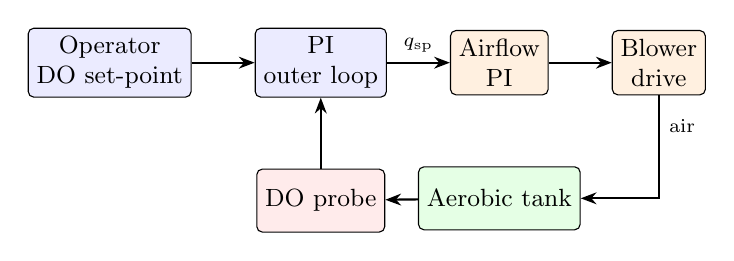
\begin{tikzpicture}[
  font=\small,
  box/.style={draw, rounded corners=2pt, align=center, minimum height=8mm, inner sep=3pt},
  arr/.style={-{Stealth[length=2mm]}, thick}
]
\node[box, fill=blue!8] (sp) {Operator\\DO set-point};
\node[box, fill=blue!8, right=8mm of sp] (pi) {PI\\outer loop};
\node[box, fill=orange!12, right=8mm of pi] (fc) {Airflow\\PI};
\node[box, fill=orange!12, right=8mm of fc] (vfd) {Blower\\drive};
\node[box, fill=green!10, below=9mm of fc] (tank) {Aerobic tank};
\node[box, fill=red!8, below=9mm of pi] (do) {DO probe};
\draw[arr] (sp) -- (pi);
\draw[arr] (pi) -- node[above,font=\scriptsize]{$q_{\mathrm{sp}}$} (fc);
\draw[arr] (fc) -- (vfd);
\draw[arr] (vfd) -- node[right,font=\scriptsize,pos=0.3]{air} (vfd |- tank) -- (tank);
\draw[arr] (tank) -- (do);
\draw[arr] (do) -- (pi);
\end{tikzpicture}
\caption{Cascade dissolved-oxygen control as it is usually installed. The outer loop does not see the production calendar, and the blower drive does not see a surge constraint from the optimizer. Both limits are outside this diagram on purpose: they are the gap Chapter~\ref{ch:method} closes.}
\label{fig:cascade-classical}
\end{figure}

\subsection{What the fan-control literature does not give a brewery}

The gap can be stated without a new slogan. Published predictive aeration controllers, including the hybrid and economic ones cited above, optimize a transfer coefficient or an airflow for a municipal load. They do not ingest a batch production schedule as a known disturbance trajectory \cite{harjunkoski2014,goode2013fouling,pettigrew2015cip}. They rarely place the centrifugal surge margin inside the same optimization as the dissolved-oxygen limit \cite{gravdahl1999surge,schraa2017}. And they treat $\alpha$ in \eqref{eq:otr} as a calibrated constant, or they hide it inside a black-box gain, which fails when the next disturbance is a detergent. The first technology of this thesis is the controller that fills that gap: a hybrid economic predictive law whose preview comes from the brewery calendar and whose fan model is \eqref{eq:header-dp}--\eqref{eq:polytropic} with an explicit surge inequality. The second technology, reviewed next, is how $\alpha$ is obtained in time to be useful to that law.

\section{Research on physics-informed sensing of oxygen transfer}
\label{sec:prev-sensor}

\subsection{Why a dissolved-oxygen probe is not an oxygen-transfer measurement}

A dissolved-oxygen probe reports $C$ in \eqref{eq:asm1-do}. It does not report $K_La$, $\alpha$, or $\mathrm{OUR}$. Those three quantities appear only as a product and a difference. Rearrangement of a steady balance, ignoring the small advective term, gives
\begin{equation}
\label{eq:unident}
K_La\,(C^{*}_{\infty}-C)
-
\mathrm{OUR}
\approx 0.
\end{equation}
Any pair $(K_La,\mathrm{OUR})$ on that line agrees with the same $C$. A single probe, at a single airflow, cannot separate a surfactant event, which lowers $K_La$, from a load event, which raises $\mathrm{OUR}$. Both make $C$ fall, and a proportional-integral fan loop responds to both by adding air. If the cause was surfactant, extra air is partly right. If the probe itself has fouled and reads low, extra air is waste. Rieger, Alex, and co-workers documented, early, that sensor properties and not only control laws decide whether automatic aeration is trustworthy \cite{rieger2003sensors,olsson2012ica}.

The direct experimental answer is off-gas testing. The oxygen mole fraction in the gas leaving the tank, compared with the air in, gives the oxygen actually transferred, and hence a field $K_La$ and a field efficiency, without assuming the biological rate \cite{redmon1983,leu2009,asce2007oxygen}. Leu, Rosso, Larson, and Stenstrom showed that real-time efficiency monitoring of this kind can be used to cut aeration energy, because the operator stops paying for transfer that the diffuser grid is no longer delivering \cite{leu2009,rosso2008state}. Off-gas hoods are the reference measurement. They are also equipment: hoods, gas sensors, and a maintenance task. A brewery polishing tank can justify them as a calibration tool. It is a weak assumption that every tank, every week, will have a clean hood signal at the moment a clean-in-place slug arrives. A soft sensor that runs on the fan instruments the plant already owns is the practical companion, checked against off-gas when the hood is in service.

\subsection{The surfactant factor}

The $\alpha$ factor is the ratio of process-water to clean-water mass transfer under otherwise matched conditions. Design values near $0.6$ are common for municipal fine-bubble tanks. Rosso and Stenstrom showed that surfactants depress $\alpha$ sharply, and that the depression is worse for fine bubbles than for coarse bubbles because the surfactant occupies the interface that fine bubbles were built to maximize \cite{rosso2006alpha}. Viscosity and high mixed-liquor solids depress transfer again, which is why high-solids tanks need their own correction \cite{krampe2003,mueller2002aeration}. Brewery clean-in-place liquors are a surfactant source by design. The detergents that remove beer stone and biofilm are the same class of molecules that sit on an air bubble \cite{goode2013fouling,pettigrew2015cip,simate2011}. In addition, brewery waste is warm and can carry diatomaceous earth fines from filtration, which abrade and clog diffuser pores and therefore move $k_{0}$ in \eqref{eq:kla-air} as well as $\alpha$ \cite{fillaudeau2006}.

A constant $\alpha$, identified during a quiet week, is then not a conservative design choice. It is an optimistic one. The fan controller that uses it will under-predict the airflow required during the detergent hour and will over-predict it afterward, if the identification is ever updated from that hour alone. The literature already knows the chemistry. It does not, in the control papers cited in Section~\ref{sec:prev-mpc}, close the loop from a live $\alpha$ estimate back into a fan optimizer on a brewery schedule.

\subsection{Soft sensors and what they have been asked to estimate}

Data-derived soft sensors for treatment plants are reviewed by Haimi, Mulas, Corona, and Vahala \cite{haimi2013soft}. The typical target is an effluent concentration that is measured in the laboratory a few times a day: chemical oxygen demand, total nitrogen, or suspended solids. The typical inputs are the online sensors the plant already has. D{\"u}rrenmatt and Gujer compared data-driven model classes for the same operational purpose and stressed that a model which fits a historical record can still be useless to an operator if its inputs are not the decisions the operator can move \cite{durrenmatt2012}. Newhart, Holloway, Hering, and Cath review performance analysis of plants from operating data, and Corominas and co-workers review the step from data to an operational decision \cite{newhart2019,corominas2018}. The shared warning is worth keeping. A soft sensor that is accurate on yesterday's file and silent about its own physics will be believed for a month and then bypassed.

For dissolved oxygen specifically, the prediction problem is easier than effluent chemical oxygen demand, because the probe exists and is simply late, noisy, or drifting. Koksal and Aydin report a hybrid of transfer learning and physics-informed modelling for dissolved-oxygen prediction on an industrial plant, using a simulator as one source of knowledge and another plant as a second source \cite{koksal2024,pan2010transfer}. That paper is the closest published neighbour of the second technology here. It improves a dissolved-oxygen forecast. It does not extract $\alpha$ as a variable to be handed to a fan optimizer, and it does not use a production schedule as an input. Those two uses are the difference this thesis claims.

Classical identification would write a small parameter vector $\theta=(\alpha,k_{0})$ and a state that includes $C$ and a slowly varying oxygen uptake, and would run a recursive estimator \cite{ljung1999,kalman1960,rao2003mhe}. Moving-horizon estimation is the constrained version of that idea and matches the constraints already present in predictive control \cite{rao2003mhe,rawlings2017mpc}. It is the right tool when the parameter dimension is small and the model is trusted. It is brittle when the airflow-to-$K_La$ exponent, the probe bias, and a sudden surfactant step are all wrong together. A physics-informed network is used here not because neural networks are newer, but because the residual of \eqref{eq:asm1-do} can be imposed on a function approximator that also accepts the schedule features a low-order parameter vector does not have room for.

\subsection{Physics-informed models}

A physics-informed neural network trains a differentiable function $u_{\phi}(x)$ so that a differential residual, not only a data error, is small \cite{raissi2019pinn,karniadakis2021piml}. For a scalar residual $r(x,u_{\phi},\partial u_{\phi})$, the training objective has the shape
\begin{equation}
\label{eq:pinn-generic}
\mathcal{L}(\phi)
=
\mathcal{L}_{\mathrm{data}}(\phi)
+
\lambda\,
\mathcal{L}_{\mathrm{phys}}(\phi)
+
\lambda_{b}\,
\mathcal{L}_{\mathrm{bound}}(\phi).
\end{equation}
Raissi, Perdikaris, and Karniadakis demonstrated the pattern on forward and inverse partial differential equations \cite{raissi2019pinn}. Karniadakis and co-workers review the wider programme of physics-informed machine learning \cite{karniadakis2021piml}. The training difficulties are now well described. Gradient conflict between the data term and the residual term produces models that fit the probe and ignore the balance, or the reverse \cite{wang2021gradient,cuomo2022}. Libraries such as DeepXDE make the residual form easy to express \cite{lu2021deepxde}. None of that work is a wastewater paper. The transferrable part is the residual. Here the residual is not a partial differential equation on a spatial mesh. It is the ordinary balance \eqref{eq:asm1-do}, evaluated on the samples the historian already stores, plus algebraic residuals from the fan map \eqref{eq:polytropic} so that a claimed airflow has to agree with the measured power.

Neural differential equations are a second, related form: the network defines a vector field and an integrator produces the trajectory \cite{chen2018node,hochreiter1997lstm,goodfellow2016deep}. They are attractive when the state must be rolled forward over a long horizon. They are heavier than this problem needs at inference time. The fan controller runs on an edge computer on a cycle of one to five minutes. A small residual network that emits $\alpha$, $K_La$, and $\mathrm{OUR}$ in one shot, trained with \eqref{eq:pinn-generic}, meets that cycle. The long short-term memory network remains relevant as a baseline for the data term, which is why it is cited, and it is not the model this thesis asks the operator to trust \cite{hochreiter1997lstm}.

Identifiability still has to be argued, because a network can hide the non-uniqueness of \eqref{eq:unident} inside its weights. The argument used in Chapter~\ref{ch:method} is structural. Airflow and power fix a delivered $q$ through \eqref{eq:polytropic}. The clean-water curve \eqref{eq:kla-air} then fixes $K_La$ up to $\alpha$. The oxygen balance fixes $\mathrm{OUR}$ once $K_La$ and $C$ are known. The schedule feature, which is zero in quiet hours and one during a detergent recipe, gives $\alpha$ a reason to move that is not collinear with a smooth diurnal uptake. When that feature is constant for a long time, the information matrix thins, and the estimator must hold $\alpha$ rather than chase noise. That is a standard excitation requirement \cite{ljung1999}, applied to a plant whose excitation is partly chosen by the production department.

\subsection{What the sensing literature does not give the fan controller}

Off-gas is accurate and scarce. Black-box soft sensors are available and unconstrained by \eqref{eq:otr}. Physics-informed dissolved-oxygen models now exist for industrial wastewater \cite{koksal2024}, and they stop at the forecast of $C$. The missing instrument is a soft sensor whose outputs are the parameters of the fan problem: a live $\alpha$, a live $K_La$, and a live uptake, with a residual that tells the controller when the dissolved-oxygen probe should not be believed. That is the second technology. It is useful only if the first technology has a place to put the numbers. The two reviews are therefore one design.

\begin{figure}[ht]
\centering
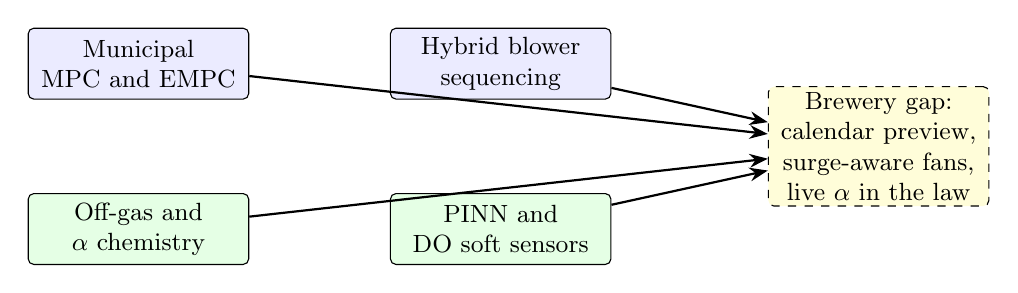
\begin{tikzpicture}[
  font=\small,
  box/.style={draw, rounded corners=2pt, align=center, minimum width=28mm, minimum height=9mm, inner sep=2pt},
  gap/.style={draw, dashed, rounded corners=2pt, align=center, minimum width=28mm, minimum height=9mm, inner sep=2pt, fill=yellow!15}
]
\node[box, fill=blue!8] (lit1) at (0,0) {Municipal\\MPC and EMPC};
\node[box, fill=blue!8] (lit2) at (4.6,0) {Hybrid blower\\sequencing};
\node[box, fill=green!10] (lit3) at (0,-2.1) {Off-gas and\\$\alpha$ chemistry};
\node[box, fill=green!10] (lit4) at (4.6,-2.1) {PINN and\\DO soft sensors};
\node[gap] (g1) at (9.4,-1.05) {Brewery gap:\\calendar preview,\\surge-aware fans,\\live $\alpha$ in the law};
\draw[-{Stealth}, thick] (lit1) -- (g1);
\draw[-{Stealth}, thick] (lit2) -- (g1);
\draw[-{Stealth}, thick] (lit3) -- (g1);
\draw[-{Stealth}, thick] (lit4) -- (g1);
\end{tikzpicture}
\caption{The four bodies of work this chapter uses, and the brewery-specific gap they leave. Chapter~\ref{ch:method} puts a schedule-aware fan controller on one side of the gap and a physics-informed transfer sensor on the other.}
\label{fig:gap}
\end{figure}

\section{Problem set}
\label{sec:problem}

\subsection{The plant the controller is responsible for}

The plant considered here is the wastewater cleaning end of a brewery, not the brewhouse. Water that has been used in production is collected, treated, and discharged. Reuse inside the brewery is outside the problem. The train, in process order, is coarse screening, a mixed and lightly aerated equalization tank, pH correction, anaerobic high-rate pretreatment, dissolved-air flotation as a solids buffer, an aerobic polishing tank with fine-bubble diffusion, and a secondary clarifier. Anaerobic pretreatment is included because brewery waste is strong enough that sending it raw to an aerobic tank makes the fan problem artificially impossible; the anaerobic stage is the standard response in the brewery treatment literature \cite{simate2011,ashraf2021,werkneh2019,shao2008asbr,chen2016anmbr,ince2000,batstone2002adm1,bernard2001,nopens2009interface}. The fans this thesis controls are the aerobic blowers and the exhaust fans on equalization and flotation. Pumps, dosing valves, and the clarifier mechanism are in the automation, and they are not the optimization variables of the two technologies.

Table~\ref{tab:train} fixes the representative sizes used from here on. They describe a polishing train after anaerobic pretreatment, sized so that a competent dissolved-oxygen loop can meet the study discharge limit, and so that a constant-speed blower sized for the worst hour wastes a large amount of air in the quiet hours. They are not the nameplate of a particular site.

\begin{table}[ht]
\centering
\caption{Representative cleaning train used as the problem data. Aerobic influent values are after anaerobic pretreatment and refer to the five production regimes of Table~\ref{tab:regimes}.}
\label{tab:train}
\begin{tabular}{@{}ll@{}}
\toprule
Quantity & Value used in this thesis \\
\midrule
Equalization & mixed, detention of several hours, exhaust fan pair \\
Aerobic volume $V$ & \SI{900}{\cubic\metre} \\
Mixed liquor $X$ & \SI{3800}{\milli\gram\per\litre} volatile solids \\
Diffusers & fine bubble, submergence giving about \SI{52}{\kilo\pascal} static head \\
Blowers & three centrifugal machines, variable speed, common header \\
Header capacity & \SI{9000}{\nmcph} \\
Mixing floor & \SI{900}{\nmcph} \\
Inert $\mathrm{COD}$ fraction $f$ & $0.08$ \\
Study discharge limit & \SI{125}{\milli\gram\per\litre} $\mathrm{COD}$ in the clarifier effluent \\
Dissolved-oxygen floor & \SI{1.5}{\milli\gram\per\litre} during production, as an operational constraint \\
\bottomrule
\end{tabular}
\end{table}

The study discharge limit of \SI{125}{\milli\gram\per\litre} chemical oxygen demand is taken as the numerical permit target inside the optimization and the estimation. It is the same order as the secondary-treatment figure used for urban wastewater in the European directive, and it is used here as a study target for a direct discharge, not as a claim that every brewery permit is that number \cite{eu1991uwwtd,tchobanoglous2014}. A site permit can be tighter or can be a sewer ordinance. The controller does not depend on the number $125$. It depends on having a number.

The five regimes in Table~\ref{tab:regimes} are the weekly disturbance. They are a compressed production calendar: a long base load, a brewhouse peak, a fermentation clean-in-place window in which $\alpha$ falls because detergent reaches the aerobic tank, a shorter packaging clean-in-place window, and a weekend hold. Durations sum to $168$ hours. Mean influent flow over the week is $55.5\,\mathrm{m^{3}/h}$ and the flow-weighted mean aerobic influent chemical oxygen demand is about \SI{402}{\milli\gram\per\litre}. Both follow from the table by direct averaging, and both are recomputed in Chapter~\ref{ch:estimate} when energy is normalized.

\begin{table}[ht]
\centering
\caption{Weekly production regimes imposed on the aerobic polishing tank. The factor $\alpha$ is the true plant value. Controllers that assume a constant $\alpha$ do not receive this column.}
\label{tab:regimes}
\begin{tabular}{@{}lrrrrrr@{}}
\toprule
Regime & Hours & $Q$ (\si{\cubic\metre\per\hour}) & $\mathrm{COD}$ (\si{\milli\gram\per\litre}) & TKN & $\alpha$ & $T$ (\si{\celsius}) \\
\midrule
Base production & 96 & 50 & 380 & 26 & 0.60 & 28 \\
Brewhouse peak & 30 & 70 & 460 & 34 & 0.52 & 31 \\
Fermentation CIP & 18 & 75 & 430 & 28 & 0.40 & 33 \\
Packaging CIP & 12 & 68 & 410 & 26 & 0.46 & 30 \\
Weekend hold & 12 & 22 & 160 & 12 & 0.66 & 26 \\
\bottomrule
\end{tabular}
\end{table}

\begin{figure}[ht]
\centering
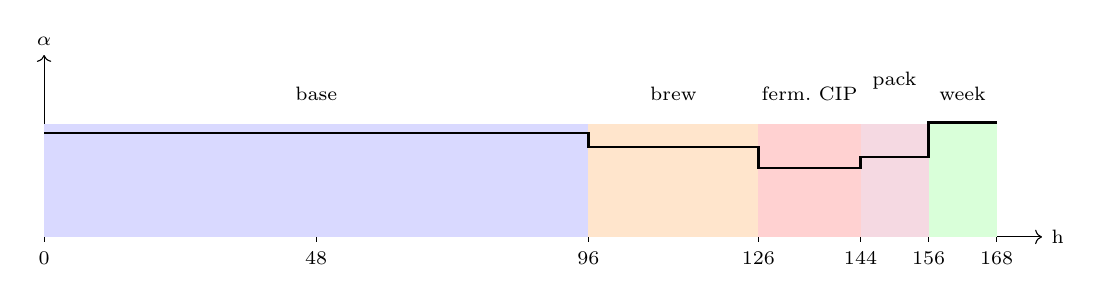
\begin{tikzpicture}[font=\scriptsize, x=0.072cm, y=0.55cm]
  \draw[->] (0,0) -- (176,0) node[right] {h};
  \draw[->] (0,0) -- (0,4.2) node[above] {$\alpha$};
  \foreach \x/\name in {0/0, 48/48, 96/96, 126/126, 144/144, 156/156, 168/168}{
    \draw (\x,0) -- (\x,-0.12) node[below, rotate=0] {\x};
  }
  \fill[blue!15] (0,0) rectangle (96,2.6);
  \fill[orange!20] (96,0) rectangle (126,2.6);
  \fill[red!18] (126,0) rectangle (144,2.6);
  \fill[purple!15] (144,0) rectangle (156,2.6);
  \fill[green!15] (156,0) rectangle (168,2.6);
  \draw[thick] (0,2.40) -- (96,2.40) -- (96,2.08) -- (126,2.08) -- (126,1.60) -- (144,1.60) -- (144,1.84) -- (156,1.84) -- (156,2.64) -- (168,2.64);
  \node at (48,3.3) {base};
  \node at (111,3.3) {brew};
  \node at (135,3.3) {ferm.\ CIP};
  \node at (150,3.6) {pack};
  \node at (162,3.3) {week};
\end{tikzpicture}
\caption{The true oxygen-transfer factor over the representative week. The drop at $126\,\mathrm{h}$ is the fermentation clean-in-place detergent reaching the aerobic tank. A controller that keeps $\alpha=0.55$ is wrong on this interval by about thirty percent.}
\label{fig:alpha-week}
\end{figure}

\subsection{Biological and oxygen balances that define feasibility}

The estimation model, stated here because the problem is not well posed without it, is a single aerobic tank with biodegradable chemical oxygen demand $S_{b}$, inert chemical oxygen demand $S_{i}$, ammonia $S_{n}$, and dissolved oxygen $C$. Mixed-liquor solids $X$ are held by sludge-age control and are an input, not a state. With Monod factors
\begin{equation}
\label{eq:monod}
\mu_{S}
=
\frac{S_{b}}{K_{S}+S_{b}},
\quad
\mu_{C}
=
\frac{C}{K_{\mathrm{DO}}+C},
\quad
\mu_{N}
=
\frac{S_{n}}{K_{N}+S_{n}},
\end{equation}
the rates used throughout this thesis are
\begin{align}
r_{\mathrm{COD}}
&=
q_{\mathrm{COD}}\,X\,\mu_{S}\,\mu_{C},
&
r_{N}
&=
q_{N}\,X\,\mu_{N}\,\mu_{C},
\label{eq:rates}
\end{align}
and the oxygen uptake that the fans must match is
\begin{equation}
\label{eq:our}
\mathrm{OUR}
=
Y_{\mathrm{O_{2},COD}}\,r_{\mathrm{COD}}
+
Y_{\mathrm{O_{2},N}}\,r_{N}.
\end{equation}
The numerical values are $K_{S}=\SI{40}{\milli\gram\per\litre}$, $K_{\mathrm{DO}}=\SI{0.35}{\milli\gram\per\litre}$, $K_{N}=\SI{1}{\milli\gram\per\litre}$, $q_{\mathrm{COD}}=0.0145\,\mathrm{L\,mg^{-1}\,h^{-1}}$, $q_{N}=0.00040\,\mathrm{L\,mg^{-1}\,h^{-1}}$, $Y_{\mathrm{O_{2},COD}}=0.95$, and $Y_{\mathrm{O_{2},N}}=4.57$. The product $q_{\mathrm{COD}}X$ is about \SI{55}{\milli\gram\per\litre\per\hour}, which is the kinetic ceiling. The fan ceiling is lower during the detergent window, and that is intentional: the interesting constraint is oxygen transfer, not a kinetic parameter.

Mass balances close the problem statement:
\begin{align}
\frac{\mathrm{d}S_{b}}{\mathrm{d}t}
&=
\frac{Q}{V}\bigl((1-f)\,\mathrm{COD}_{\mathrm{in}}-S_{b}\bigr)
-
r_{\mathrm{COD}},
\label{eq:sb}\\
\frac{\mathrm{d}S_{i}}{\mathrm{d}t}
&=
\frac{Q}{V}\bigl(f\,\mathrm{COD}_{\mathrm{in}}-S_{i}\bigr),
\label{eq:si}\\
\frac{\mathrm{d}S_{n}}{\mathrm{d}t}
&=
\frac{Q}{V}\bigl(\mathrm{TKN}_{\mathrm{in}}-S_{n}\bigr)
-
r_{N},
\label{eq:sn}\\
\frac{\mathrm{d}C}{\mathrm{d}t}
&=
K_La(\alpha,q,T)\,
\bigl(\beta C^{*}(T)-C\bigr)
-
\mathrm{OUR}.
\label{eq:do-bal}
\end{align}
Effluent chemical oxygen demand is $S_{b}+S_{i}$ after the clarifier has removed solids. The clarifier itself is not dynamically modelled. The Tak{\'a}cs clarifier would be the next model if the permit were on suspended solids rather than on dissolved and colloidal organic load \cite{takacs1991}. For this problem the clarifier is a solids separator that the automation must keep in service, and the organic permit is decided in the aerobic tank.

The transfer coefficient in \eqref{eq:do-bal} is the estimation curve
\begin{equation}
\label{eq:kla-est}
K_La
=
\alpha\,
k_{\mathrm{ref}}
\left(\frac{q}{q_{\mathrm{ref}}}\right)^{0.82}
\theta^{\,T-20},
\end{equation}
with $k_{\mathrm{ref}}=6.5\,\mathrm{h^{-1}}$ at $q_{\mathrm{ref}}=\SI{2500}{\nmcph}$ and $\theta=1.024$. Saturation $C^{*}(T)$ is interpolated from the fresh-water table $8.11$, $7.83$, $7.54$, $7.43$, $7.16\,\mathrm{mg/L}$ at $26$, $28$, $30$, $31$, and \SI{33}{\celsius}. The factor $\beta$ is $0.95$. These numbers are part of the problem data. Changing them changes the absolute kilowatt-hours and should not change the ranking of a schedule-aware law against a law that ignores the schedule, which is the comparison Chapter~\ref{ch:estimate} is built to make.

Fan power is \eqref{eq:polytropic} with the header
\begin{equation}
\label{eq:dp-num}
\Delta p
=
52
+
0.55\left(\frac{q}{1000}\right)^{2}
\quad[\mathrm{kPa}],
\end{equation}
inlet temperature \SI{20}{\celsius}, and $\eta=0.70\times 0.95\times 0.97$. Delivered airflow lags the command with a time constant of $0.10\,\mathrm{h}$, and the probe lags the tank with a time constant of $0.08\,\mathrm{h}$. Those lags are why a purely reactive loop is late, and why a preview of forty-five minutes is long enough to matter.

One steady-state check belongs in the problem statement so that later plots are not the first time the numbers appear. At base load, $Q=\SI{50}{\cubic\metre\per\hour}$, $\mathrm{COD}_{\mathrm{in}}=\SI{380}{\milli\gram\per\litre}$, $f=0.08$, the biodegradable influent is \SI{350}{\milli\gram\per\litre}. With $C=\SI{1.8}{\milli\gram\per\litre}$ the Monod product is high enough that the balance \eqref{eq:sb} settles near $S_{b}\approx\SI{25}{\milli\gram\per\litre}$. Inert chemical oxygen demand settles at $f\,\mathrm{COD}_{\mathrm{in}}=\SI{30}{\milli\gram\per\litre}$. Effluent chemical oxygen demand near \SI{55}{\milli\gram\per\litre} is then the quiet-week target, not a result to be celebrated. The fermentation clean-in-place window, with the same kinetic ceiling and $\alpha=0.40$, settles near \SI{90}{\milli\gram\per\litre} if dissolved oxygen stays near \SI{2}{\milli\gram\per\litre}, and it climbs through the \SI{125}{\milli\gram\per\litre} study limit if dissolved oxygen is held near \SI{0.5}{\milli\gram\per\litre} for a large part of the eighteen hours. The controller's job is to buy the first of those two outcomes with as little fan energy as the surge and mixing constraints allow.

\subsection{The two decision problems}

The technologies are now stated as optimization problems. Time is discrete with step $\Delta t$. The horizon is $N$ steps. The schedule encoder, defined properly in Chapter~\ref{ch:method}, produces a disturbance preview $D_{k:k+N}$ that contains future flow, chemical oxygen demand, temperature, and a detergent flag.

\textbf{Problem P1, fan control.} Given the current state estimate and the preview $D$, choose the binary staging $z_{0:N-1}$ and the continuous commands $u_{0:N-1}$ (fan speeds and the total airflow) to minimize
\begin{equation}
\label{eq:p1}
\sum_{j=0}^{N-1}
\left(
P(q_{j},z_{j})\,\Delta t
+
\lambda_{C}\,\phi_{C}(C_{j})
+
\lambda_{S}\,\phi_{S}(S_{b,j}+S_{i,j})
+
\lambda_{z}\,\abs{z_{j}-z_{j-1}}
\right)
\end{equation}
subject to the discrete form of \eqref{eq:sb}--\eqref{eq:do-bal}, the fan map, the surge inequalities, the box limits on speed and airflow, and the probe-health interlock. The hinge penalties $\phi_{C}$ and $\phi_{S}$ are zero when dissolved oxygen is above its floor and chemical oxygen demand is below the study limit, and they grow linearly beyond those lines. This is an economic predictive problem in the sense of \cite{zeng2015empc,ellis2014empc,rawlings2017mpc}, with a hybrid decision in the sense of \cite{bemporad1999hybrid,cristea2011}.

\textbf{Problem P2, transfer sensing.} Given a window of fan power, airflow, temperature, header pressure, dissolved oxygen, and the same schedule features, choose the network parameters $\phi$ and the latent trajectories of $\alpha$, $K_La$, and $\mathrm{OUR}$ to minimize \eqref{eq:pinn-generic}, where the physics term is the residual of \eqref{eq:do-bal} and a power residual from \eqref{eq:polytropic}. The deployed sensor freezes $\phi$ and runs a short update of the latent state only. P2 is useful insofar as its $\alpha$ and $K_La$ reduce the model error inside P1. A sensor that predicts dissolved oxygen accurately and emits an $\alpha$ the optimizer cannot use has not solved P2 as defined here.

\subsection{Questions the rest of the thesis has to answer}

The design questions are the following.

\begin{enumerate}[leftmargin=1.6em,itemsep=0.4em]
\item Can the production calendar be encoded as a disturbance trajectory that a fan optimizer accepts without a human redrawing set-points at the start of each clean-in-place?
\item Can the blower staging, the surge margin, and the header power model sit inside that optimizer rather than in a separate sequencer that fights it?
\item Can $\alpha$ during a detergent window be estimated from instruments the fan already has, with the oxygen balance enforced, well enough that the optimizer stops using the quiet-week value?
\item On the representative week of Table~\ref{tab:regimes}, how much blower energy does the combined law use relative to constant speed, to a competent dissolved-oxygen proportional-integral loop at a fixed set-point of \SI{2.5}{\milli\gram\per\litre}, and to a predictive inversion that keeps $\alpha$ at $0.55$ and does not read the calendar?
\item Which of those savings survive the mixing floor, the blower lag, and a soft-sensor lag of a few tenths of an hour?
\end{enumerate}

The questions are system questions. They are answered by a specification in Chapter~\ref{ch:method} and by an integration of \eqref{eq:sb}--\eqref{eq:do-bal} in Chapter~\ref{ch:estimate}. They are not answered by a claim of a field trial. A field trial would need a brewery, a permit, and an off-gas campaign this document does not contain.

\subsection{Assumptions that bound the problem}

The assumptions are stated so they can be attacked. Solids inventory $X$ is constant over the week. The clarifier does not limit the organic result. Anaerobic pretreatment has already happened, and its upsets appear only as the influent columns of Table~\ref{tab:regimes}. The production calendar is known forty-five minutes ahead with the correct recipe identity. A wrong recipe is a different experiment and is named as such in the estimation. The dissolved-oxygen probe is biased only within the lag model, except in the fault discussion of the soft sensor, where a stuck probe is considered separately. Electricity price is constant inside the week, so economic optimization coincides with energy minimization plus constraint penalties. Ambient air density is fixed at the inlet temperature used in \eqref{eq:polytropic}. Exhaust fans follow a speed schedule tied to the same regimes and are metered, but they are not decision variables of P1. Their energy is reported so the fan account is complete.

Under those assumptions the plant is controllable in the limited sense that there exist airflow trajectories, inside the header capacity, that keep the study chemical-oxygen-demand limit on every regime of Table~\ref{tab:regimes} if dissolved oxygen is held near the set-points of Chapter~\ref{ch:method}. The constant-speed policy that meets the worst regime also meets the limit, at a power that the quiet hours do not need. The engineering problem is the difference between those two facts.

\subsection{How this problem sits against the published controllers}

Table~\ref{tab:litmap} is the operational summary of Section~\ref{sec:prev-mpc} and Section~\ref{sec:prev-sensor}. A row is included only if the paper is part of the argument, not as a census. The columns are the ones that decide whether the paper already solves P1 and P2. None of the rows has a yes in both the calendar column and the live-$\alpha$ column. That empty intersection is the problem set.

\begin{table}[ht]
\centering
\caption{What the cited control and sensing results provide, relative to problems P1 and P2. ``Airflow'' means the decision is a smooth transfer coefficient or a flow, not a staged centrifugal fan.}
\label{tab:litmap}
\small
\begin{tabular}{@{}p{3.3cm}p{2.3cm}p{2.4cm}p{2.2cm}p{2.4cm}@{}}
\toprule
Source & Plant disturbance & Actuator & Live $\alpha$ & Calendar preview \\
\midrule
Holenda et al.\ \cite{holenda2008} & benchmark DO & airflow & no & no \\
Shen et al.\ \cite{shen2008} & BSM1 file & airflow & no & no \\
Cristea et al.\ \cite{cristea2011} & plant DO & hybrid air & no & no \\
Ostace et al.\ \cite{ostace2011} & benchmark & airflow & no & no \\
Zeng and Liu \cite{zeng2015empc} & BSM1 file & airflow & no & no \\
Sant{\'i}n et al.\ \cite{santin2015jpc} & benchmark & DO set-point & no & no \\
Leu et al.\ \cite{leu2009} & municipal & off-gas & measured & no \\
Koksal and Aydin \cite{koksal2024} & industrial DO & forecast of $C$ & not emitted & no \\
This thesis & Table~\ref{tab:regimes} & staged fans & sensor & recipe clock \\
\bottomrule
\end{tabular}
\end{table}

The table also fixes a scope mistake that is easy to make when reading brewery wastewater reviews. Simate and co-workers, Fillaudeau and co-workers, Werkneh and co-workers, and Ashraf and co-workers describe treatment trains, reuse options, and anaerobic energy recovery \cite{simate2011,fillaudeau2006,werkneh2019,ashraf2021,shao2008asbr,chen2016anmbr}. Those reviews are why the train in Figure~\ref{fig:train} has an anaerobic stage and why the water is discharged rather than returned to the brewhouse. They are not fan-control papers. Using them as if they had already optimized blower speed would invent a literature that does not exist. The control citations and the brewery citations meet only in the problem statement of this chapter: the disturbance shape comes from the brewery reviews, and the mathematics that can accept that shape comes from the predictive-control papers, which have not yet been given it.

A short oxygen budget shows why the anaerobic stage is inside the problem boundary rather than outside it. Brewery raw waste is commonly reported with chemical oxygen demand of several thousand milligrams per litre \cite{simate2011,fillaudeau2006}. At \SI{3000}{\milli\gram\per\litre}, \SI{70}{\cubic\metre\per\hour}, and one kilogram of oxygen per kilogram of chemical oxygen demand removed, the aerobic duty would be about \SI{210}{\kilo\gram\per\hour} of oxygen before any surfactant penalty. With a field transfer efficiency near ten percent and \SI{0.3}{\kilo\gram} of oxygen per normal cubic metre of air, the header would need on the order of \SI{7000}{\nmcph} even before $\alpha$ falls, and several times that during a detergent hour. That header is a different machine from the polishing header specified here. The problem in this thesis starts after anaerobic removal has already cut the aerobic influent to the hundreds of milligrams per litre in Table~\ref{tab:regimes}. The fans are still the dominant electrical load of the polishing step. They are not asked to oxidize raw beer waste.

The same budget fixes the performance indices that later chapters are allowed to quote. Effluent quality on this plant is hours above \SI{125}{\milli\gram\per\litre} chemical oxygen demand, mean effluent chemical oxygen demand, and the minimum dissolved oxygen in each regime. Energy is blower kilowatt-hours, with exhaust kilowatt-hours reported beside them and not inside them. A single weighted index in the style of the BSM effluent quality index would hide a legal chemical-oxygen-demand week inside a nitrogen term this permit does not use \cite{copp2002cost,vanrolleghem2002,nopens2010bsm2}. The indices stay separate so that a loop which saves energy by spending the dissolved-oxygen floor cannot be summarized as an improvement.

\subsection{A numerical transfer example before any controller is chosen}

The formulae \eqref{eq:otr} and \eqref{eq:kla-air} are easier to distrust when they stay symbolic. One base-regime point is computed here and then left alone. Take clean-water $K_La_{20}=4.0\,\mathrm{h^{-1}}$ at the airflow of interest, $\alpha=0.60$, $\beta=0.95$, $T=\SI{28}{\celsius}$, $\theta=1.024$, $C=\SI{1.8}{\milli\gram\per\litre}$, and $C^{*}_{28}=7.83\,\mathrm{mg/L}$. The temperature factor is $1.024^{8}$. Using $1.024^{2}\approx 1.0486$ and squaring twice gives $1.024^{8}\approx 1.209$. Then
\begin{equation}
\begin{aligned}
\mathrm{OTR}
&=
0.60\times 4.0\times\big(0.95\times 7.83-1.8\big)\times 1.209
\\
&=
2.40\times(7.44-1.8)\times 1.209
\\
&=
2.40\times 5.64\times 1.209
=
16.4\,\mathrm{mg\,L^{-1}\,h^{-1}}.
\end{aligned}
\end{equation}
Sixteen milligrams per litre per hour is the oxygen the fans are delivering at that point, not the power they draw. If the uptake is higher than $16.4$, dissolved oxygen falls until the driving force widens or the controller adds air. If a detergent moves $\alpha$ from $0.60$ to $0.40$ and nothing else changes, the transfer rate falls by the same ratio, to $16.4\times 0.40/0.60=10.9\,\mathrm{mg\,L^{-1}\,h^{-1}}$. The missing $5.5\,\mathrm{mg\,L^{-1}\,h^{-1}}$ is the entire local effect of the surfactant. No later controller creates oxygen that this product does not allow. Controllers only choose the airflow that sets $K_La_{20}$, and they only choose it well if they know which $\alpha$ to use.

The same point fixes a bound that is easy to violate in a soft sensor that is trained only on dissolved oxygen. Suppose the network reports $\alpha=0.60$ during the detergent and lowers the uptake by $5.5\,\mathrm{mg\,L^{-1}\,h^{-1}}$ to keep the balance. The dissolved-oxygen forecast can still be accurate. The fan command, which needs $\alpha$, will be wrong by the factor computed in Section~\ref{sec:openloop}. Accuracy on $C$ is not accuracy on the actuator. That is why problem P2 asks for $\alpha$, $K_La$, and uptake as separate outputs, and why the curve residual in the sensor loss is not an optional regularizer. It is the constraint that stops a good forecast from authorizing a bad fan command.

The example also bounds the exhaust fans, so they are not forgotten in a chapter about blowers. Two exhaust machines at \SI{7.5}{\kilo\watt} each, running at a speed fraction of $0.75$, draw $15\times 0.75^{3}=6.3\,\mathrm{kW}$. Over the ninety-six hours of base production that is about \SI{610}{\kilo\watt\hour}. The aerobic blower at the same hours, once it is allowed to leave constant speed, is several thousand kilowatt-hours. The exhaust fans matter for odor and for the automation interlock. They do not change which blower law is worth writing. The problem set is therefore intentionally asymmetric: both fan duties are in the plant, and only the blowers are in P1.

\chapter{Schedule-Aware Fan Control and Physics-Informed Oxygen-Transfer Sensing}
\label{ch:method}

The two technologies are specified in this chapter at the level an automation engineer can implement and a numerical estimator can test. Section~\ref{sec:saempc} is the fan controller. Section~\ref{sec:piots} is the transfer sensor. They share a clock, a schedule message, and a parameter handshake. Neither is a replacement for the safety interlocks in the programmable controller. Those interlocks are part of the system build in Chapter~\ref{ch:estimate} and are listed here only where the optimizer must know that a command will be rejected.

\section{Schedule-aware hybrid economic control of the fan cluster}
\label{sec:saempc}

\subsection{Role in the automation}

The controller sits above the blower drives and the zone airflow valves. It does not modulate a silicon-controlled rectifier on a millisecond clock. It publishes, once per minute, a staging word and an airflow set-point. Inner proportional-integral loops, of the form already reviewed in \eqref{eq:pi}, move the drives and the valves. This split is the hierarchical pattern of Brdys and of industrial model predictive control \cite{brdys2008,qin2003mpc,engell2007}. The novelty is the content of the minute-scale problem: the disturbance is a brewery calendar, the stage cost is fan kilowatt-hours plus discharge and surge penalties, and the transfer coefficient inside the prediction is the live output of Section~\ref{sec:piots}.

Figure~\ref{fig:arch} shows the data the optimizer is allowed to see. The production schedule is a message, not a guess. The soft sensor is a message. Dissolved oxygen, header pressure, and power are measurements. Everything else is a model.

\begin{figure}[ht]
\centering
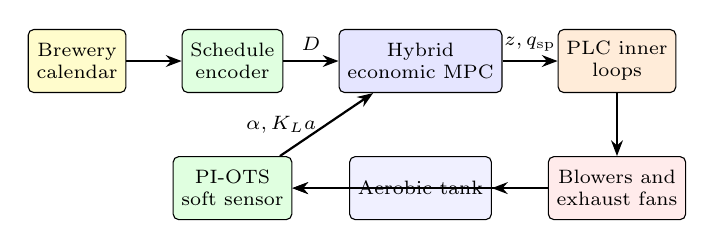
\begin{tikzpicture}[
  font=\small,
  box/.style={draw, rounded corners=2pt, align=center, minimum height=8mm, inner sep=3pt, font=\scriptsize},
  arr/.style={-{Stealth[length=2mm]}, thick}
]
\node[box, fill=yellow!20] (cal) {Brewery\\calendar};
\node[box, fill=green!12, right=7mm of cal] (enc) {Schedule\\encoder};
\node[box, fill=blue!10, right=7mm of enc] (mpc) {Hybrid\\economic MPC};
\node[box, fill=orange!15, right=7mm of mpc] (plc) {PLC inner\\loops};
\node[box, fill=red!8, below=8mm of plc] (fans) {Blowers and\\exhaust fans};
\node[box, fill=green!12, below=8mm of enc] (soft) {PI-OTS\\soft sensor};
\node[box, fill=blue!6, below=8mm of mpc] (tank) {Aerobic tank};
\draw[arr] (cal) -- (enc);
\draw[arr] (enc) -- node[above,font=\scriptsize]{$D$} (mpc);
\draw[arr] (mpc) -- node[above,font=\scriptsize]{$z,q_{\mathrm{sp}}$} (plc);
\draw[arr] (plc) -- (fans);
\draw[arr] (fans) -- (tank);
\draw[arr] (tank) -- (soft);
\draw[arr] (soft) -- node[left,font=\scriptsize]{$\alpha,K_La$} (mpc);
\draw[arr] (fans) -- (soft);
\end{tikzpicture}
\caption{Information pattern of the schedule-aware controller. The calendar and the soft sensor are inputs. The programmable controller remains the only device that talks to the drives.}
\label{fig:arch}
\end{figure}

\subsection{Schedule encoder}

A brewery schedule is a list of batches and clean-in-place recipes with planned start times \cite{isa95,harjunkoski2014,pettigrew2015cip,goode2013fouling}. The encoder does not optimize that list. It maps each recipe class onto a disturbance segment. The classes used here are the five regimes of Table~\ref{tab:regimes}. A site implementation would use the site's recipe identifiers and a table maintained with the production department. The mathematics does not change.

Let the planned regime at future time $t_{k}+j\Delta t$ be $\rho_{k+j}$. The preview vector is
\begin{equation}
\label{eq:preview}
D_{k+j}
=
\big(
Q(\rho_{k+j}),\;
\mathrm{COD}(\rho_{k+j}),\;
T(\rho_{k+j}),\;
\delta_{\mathrm{CIP}}(\rho_{k+j})
\big),
\end{equation}
where $\delta_{\mathrm{CIP}}$ is $1$ for a detergent recipe and $0$ otherwise. The encoder also emits the dissolved-oxygen set-point the economic layer would otherwise have to discover,
\begin{equation}
\label{eq:dosp}
C_{\mathrm{sp}}(\rho)
=
\begin{cases}
1.8 & \text{base production},\\
2.0 & \text{brewhouse peak or packaging CIP},\\
2.2 & \text{fermentation CIP},\\
1.3 & \text{weekend hold}.
\end{cases}
\end{equation}
These numbers are not magic. They sit above the operational floor of \SI{1.5}{\milli\gram\per\litre} during any production regime, they rise when Table~\ref{tab:regimes} says the load and the surfactant arrive together, and they fall on the weekend because the mixing floor, not the uptake, will set the airflow. A higher-layer optimizer can replace \eqref{eq:dosp}. In this thesis the table is the higher layer, and it is justified by the steady-state check in Section~\ref{sec:problem}: each of these set-points, with the true $\alpha$, lands effluent chemical oxygen demand under the study limit. Holding \SI{2.5}{\milli\gram\per\litre} at all times, which is the operator habit encoded in the proportional-integral baseline, buys a smaller driving force and therefore more air for the same uptake.

The preview is applied $0.75\,\mathrm{h}$ ahead of the regime boundary so that the blower lag of $0.10\,\mathrm{h}$ and the dissolved-oxygen probe lag of $0.08\,\mathrm{h}$ are already inside the lead. A calendar error of that order is a timing error, not a recipe error. Recipe identity is assumed correct in the nominal estimation. When the identity is wrong, $\delta_{\mathrm{CIP}}$ is wrong, $\alpha$ is wrong in the prediction, and the controller falls back toward the behaviour of the fixed-$\alpha$ law. That fallback is a required property, not a failure mode to be hidden.

\subsection{Prediction model inside the horizon}

The horizon model is the forward Euler form of \eqref{eq:sb}--\eqref{eq:do-bal} with step $\Delta t=1\,\mathrm{min}$ for the optimizer and a finer step only in the estimation integrator of Chapter~\ref{ch:estimate}. Writing $x=(S_{b},S_{i},S_{n},C)$,
\begin{equation}
\label{eq:euler}
x_{j+1}
=
x_{j}
+
\Delta t\,
f\!\left(x_{j}, q_{j}, \alpha_{j}, D_{k+j}\right).
\end{equation}
The transfer coefficient is \eqref{eq:kla-est} evaluated at the sensed $\alpha$ if the soft sensor is healthy and at the schedule-class default of Table~\ref{tab:regimes} if the sensor has declared itself invalid. The two sources are not averaged blindly. The rule is
\begin{equation}
\label{eq:alpha-fuse}
\alpha_{j}
=
\begin{cases}
\alpha_{\mathrm{sensor}} & \text{if } h_{\mathrm{sensor}}=1,\\[0.3em]
\alpha_{\mathrm{table}}(\rho_{k+j}) & \text{if } h_{\mathrm{sensor}}=0,
\end{cases}
\end{equation}
where $h_{\mathrm{sensor}}$ is the health bit of Section~\ref{sec:piots}. A convex combination would let a failing sensor drag a good table, which is the wrong direction of trust during a detergent window.

Power along the horizon is \eqref{eq:polytropic} with \eqref{eq:dp-num}. Staging enters by splitting the header flow across $n_{j}$ identical machines,
\begin{equation}
\label{eq:split}
q_{\mathrm{each},j}
=
\frac{q_{j}}{n_{j}},
\qquad
n_{j}
=
\sum_{i=1}^{3} z_{j,i},
\qquad
z_{j,i}\in\{0,1\}.
\end{equation}
Identical speeds are imposed. Unequal speeds on a common header fight, and the fight is not worth a few percent of efficiency on a three-machine plant \cite{dixon2014turbo}. The surge constraint is written on each online machine. With a rated flow of \SI{2800}{\nmcph} and a surge flow at $22\%$ of rated, scaled by speed through the fan law \eqref{eq:fanlaws},
\begin{equation}
\label{eq:surge}
q_{\mathrm{each},j}
\ge
1.15\,
q_{\mathrm{surge}}
\left(\frac{\omega_{j}}{\omega_{\mathrm{rated}}}\right)
\qquad
\text{for every } i \text{ with } z_{j,i}=1.
\end{equation}
The factor $1.15$ is the margin. It is a design choice, not an identified constant. A machine that the optimizer would run below that line is switched off and its flow is given to the machines that remain, or the problem is declared infeasible and the last feasible staging is held. Infeasibility handling is specified in the real-time section below, because a predictive controller that returns ``infeasible'' and then goes silent is worse than the proportional-integral loop it replaced.

Header capacity, mixing, and motor limits are
\begin{equation}
\label{eq:boxes}
q_{\min}
\le
q_{j}
\le
q_{\max},
\qquad
0
\le
\omega_{j}
\le
\omega_{\max},
\qquad
P(q_{j},n_{j})
\le
P_{\max}.
\end{equation}
On this plant $q_{\min}=\SI{900}{\nmcph}$ and $q_{\max}=\SI{9000}{\nmcph}$. The mixing floor is also a surge policy: one machine at \SI{900}{\nmcph} is above $1.15$ times the idle surge flow, so the weekend solution is legal. Two machines sharing \SI{900}{\nmcph} would not be. The optimizer must be allowed to turn machines off. A sequencer that forces all installed machines to run will make \eqref{eq:surge} infeasible on the weekend and will train the operator to bypass the optimizer.

\begin{figure}[ht]
\centering
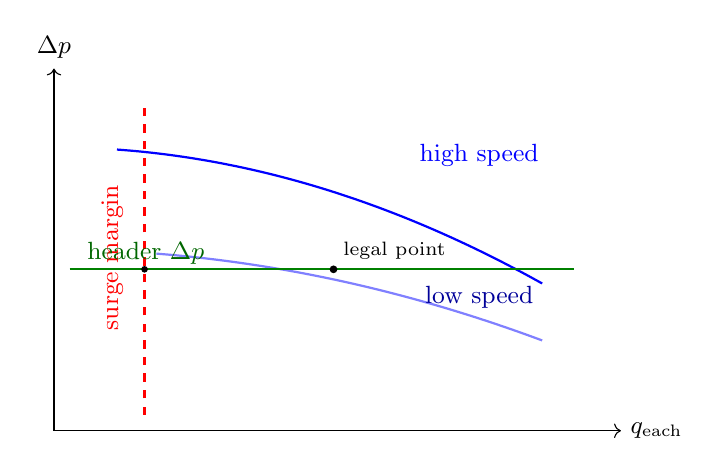
\begin{tikzpicture}[font=\small, scale=1.0]
  \draw[->] (0,0) -- (7.2,0) node[right] {$q_{\mathrm{each}}$};
  \draw[->] (0,0) -- (0,4.6) node[above] {$\Delta p$};
  \draw[domain=0.8:6.2, smooth, variable=\x, thick, blue] plot ({\x},{3.6-0.045*\x*\x});
  \draw[domain=1.3:6.2, smooth, variable=\x, thick, blue!50] plot ({\x},{2.3-0.030*\x*\x});
  \draw[dashed, red, thick] (1.15,0.2) -- (1.15,4.2);
  \node[red, rotate=90, anchor=south] at (1.0,2.2) {surge margin};
  \node[blue] at (5.4,3.5) {high speed};
  \node[blue!60!black] at (5.4,1.7) {low speed};
  \draw[thick, green!50!black] (0.2,2.05) -- (6.6,2.05);
  \node[green!40!black, anchor=west] at (0.3,2.25) {header $\Delta p$};
  \fill (3.55,2.05) circle (1.4pt) node[above right, font=\scriptsize] {legal point};
  \fill (1.15,2.05) circle (1.2pt);
\end{tikzpicture}
\caption{Sketch of the centrifugal map against a nearly flat header pressure. The legal operating point is the intersection to the right of the surge margin. Speed is raised until that intersection supplies the airflow the oxygen balance requires.}
\label{fig:fanmap}
\end{figure}

\subsection{Economic stage cost}

The cost whose sum is minimized was written as \eqref{eq:p1}. The pieces are defined here so the weights are not anonymous. Power is in kilowatts, so the first term is kilowatt-hours over the step. The dissolved-oxygen hinge is
\begin{equation}
\label{eq:hinge-c}
\phi_{C}(C)
=
\max\!\big(0,\; C_{\mathrm{floor}}(\rho)-C\big),
\end{equation}
with $C_{\mathrm{floor}}=1.5\,\mathrm{mg/L}$ in production regimes and $1.0\,\mathrm{mg/L}$ on the weekend, when the tank is only being kept from going septic. The discharge hinge is
\begin{equation}
\label{eq:hinge-s}
\phi_{S}(S)
=
\max\!\big(0,\; S-125\big),
\end{equation}
in milligrams per litre of chemical oxygen demand. The staging term counts machine starts and stops. Weights used in the specification are $\lambda_{C}=40\,\mathrm{kWh}$ per $(\mathrm{mg/L})$ per hour, $\lambda_{S}=80\,\mathrm{kWh}$ per $(\mathrm{mg/L})$ per hour, and $\lambda_{z}=8\,\mathrm{kWh}$ per machine transition. They are not electricity. They are the relative price of a constraint violation inside the optimizer, chosen so that a persistent \SI{10}{\milli\gram\per\litre} chemical-oxygen-demand violation is more expensive than the fan power available on this header, and so that a start is cheaper than an hour of surge-avoiding extra air. A site would retune $\lambda$ with its permit fine and its maintenance cost. The structure of \eqref{eq:p1} does not depend on the retune \cite{ellis2014empc,zeng2015empc,stare2007}.

Offset-free behaviour under a constant sensor bias is obtained by a bias state $b_{k}$ on the airflow command,
\begin{equation}
\label{eq:bias}
b_{k+1}
=
b_{k}
+
\Delta t\,
K_{b}\,\big(C_{\mathrm{sp}}-C^{\mathrm{meas}}_{k}\big),
\qquad
\abs{b_{k}}\le b_{\max},
\end{equation}
with $K_{b}=0.55\,\mathrm{h^{-1}}$ and $b_{\max}=0.25$ as a relative airflow trim. This is the integrator that Pannocchia and Rawlings require for offset-free predictive control, implemented as an outer bias because the deployed law in Section~\ref{sec:deployed} is a single-step inversion rather than a full nonlinear program at every minute \cite{pannocchia2003offset}. The bias is clamped so a stuck probe cannot integrate the fans to the header limit. The clamp is also the probe-fault path: if the soft sensor raises a fault, $K_{b}$ is set to zero and $q$ is frozen at the last healthy command until an operator acknowledges.

\subsection{Deployed real-time law}
\label{sec:deployed}

A three-machine hybrid problem over a two-hour horizon is a mixed-integer nonlinear program. It is solvable at a one-minute cycle with a modern interior-point solver and a short candidate list of stagings \cite{wachter2006ipopt,andersson2019casadi,bemporad1999hybrid,nocedal2006}. The estimation in Chapter~\ref{ch:estimate} does not call that solver. It integrates the deployed law that the solver reduces to when the staging list is a rule and the horizon is represented by a load scale. Publishing both, and saying which one produced the tables, is required for the numbers to be reproducible.

The deployed law at each minute is the following. Measure dissolved oxygen through the probe lag. Read $\alpha$ from the soft sensor with its own lag of $0.30\,\mathrm{h}$ and a two-percent scale caution. Look $0.75\,\mathrm{h}$ ahead on the calendar. Set the set-point to the maximum of the current regime and the previewed regime, which raises the set-point before a clean-in-place and does not lower it early. Let $L=Q\,\mathrm{COD}$ be the mass load. Apply
\begin{equation}
\label{eq:scale}
\sigma
=
\mathrm{clip}\!\left(
\frac{L_{k+0.75\,\mathrm{h}}}{L_{k}},\;
1,\;
1.35
\right)
\end{equation}
and invert the oxygen balance for the airflow that meets $\sigma\,\mathrm{OUR}$ at the set-point, using the fused $\alpha$:
\begin{equation}
\label{eq:invert}
K_La^{\star}
=
\frac{\sigma\,\mathrm{OUR}}{\beta C^{*}(T)-C_{\mathrm{sp}}},
\qquad
q^{\star}
=
q_{\mathrm{ref}}
\left(
\frac{K_La^{\star}}{\alpha\,k_{\mathrm{ref}}\,\theta^{\,T-20}}
\right)^{1/0.82}.
\end{equation}
The command is then $q=(1+b)\,q^{\star}$, clipped to $[q_{\min},q_{\max}]$, and passed through the blower lag. Staging is the rule
\begin{equation}
\label{eq:stage-rule}
n
=
\begin{cases}
1 & \text{if } q < 2600\,\mathrm{Nm^{3}/h},\\
2 & \text{if } 2600 \le q < 5200\,\mathrm{Nm^{3}/h},\\
3 & \text{otherwise},
\end{cases}
\end{equation}
rejected and increased by one machine if \eqref{eq:surge} fails. Equation~\eqref{eq:invert} is the explicit inverse of \eqref{eq:kla-est}. It is cheap, it uses the schedule through $\sigma$ and through $C_{\mathrm{sp}}$, and it uses the soft sensor through $\alpha$. It is the form whose week-long integral is reported later. The full horizon problem \eqref{eq:p1} remains the specification a solver-based implementation has to meet. On this plant the rule \eqref{eq:stage-rule} matches the surge-feasible optimum of the integer part at every regime boundary we checked by enumeration, because the three machines are identical. Enumeration is honest when there are three machines. It stops being honest when the header has machines of different sizes. That case needs the integer program, not the rule.

\begin{algorithm}[ht]
\caption{Deployed schedule-aware fan step}
\label{alg:deployed}
\KwIn{measured $C$, estimated $\mathrm{OUR}$ and $\alpha$, calendar $D$, bias $b$}
\KwOut{command $q$, staging $n$, updated bias}
$\rho \leftarrow$ current regime, $\rho^{+} \leftarrow$ regime at $t+0.75\,\mathrm{h}$\;
$C_{\mathrm{sp}} \leftarrow \max\{C_{\mathrm{sp}}(\rho), C_{\mathrm{sp}}(\rho^{+})\}$\;
$\alpha \leftarrow$ fused value from \eqref{eq:alpha-fuse}, with sensor lag\;
$\sigma \leftarrow$ load scale \eqref{eq:scale}\;
$q^{\star} \leftarrow$ inversion \eqref{eq:invert}\;
$b \leftarrow \mathrm{clip}(b + \Delta t\, K_{b}(C_{\mathrm{sp}}-C),\,-0.2,\,0.25)$\;
$q \leftarrow \mathrm{clip}((1+b)\,q^{\star},\, q_{\min},\, q_{\max})$\;
$n \leftarrow$ staging \eqref{eq:stage-rule}, increased until \eqref{eq:surge} holds\;
\Return{$q,n,b$}\;
\end{algorithm}

\subsection{A worked inversion}

The inversion is short enough to do by hand for the base regime, and the hand result is the check on the code. Take $\mathrm{OUR}=\SI{18}{\milli\gram\per\litre\per\hour}$, which is the order of the base uptake, $C_{\mathrm{sp}}=1.8$, $T=28$, $\alpha=0.60$, $\beta C^{*}=0.95\times 7.83=7.44$, and driving force $7.44-1.8=5.64$. Then
\begin{equation}
K_La^{\star}
=
18/5.64
=
3.19\,\mathrm{h^{-1}}.
\end{equation}
The temperature factor is $1.024^{8}\approx 1.21$, so
\begin{equation}
\alpha\,k_{\mathrm{ref}}\,\theta^{\,T-20}
=
0.60\times 6.5\times 1.21
=
4.72\,\mathrm{h^{-1}}.
\end{equation}
The airflow ratio to the power $0.82$ is $3.19/4.72=0.676$, and
\begin{equation}
\frac{q}{2500}
=
0.676^{\,1/0.82}
=
0.676^{\,1.220}
\approx
0.62,
\end{equation}
hence $q\approx\SI{1550}{\nmcph}$. One machine, well clear of surge, is the staging. Power from \eqref{eq:polytropic} and \eqref{eq:dp-num} at this flow is a few tens of kilowatts, not the header maximum. The same arithmetic at fermentation clean-in-place, with $\alpha=0.40$, $T=33$, and a higher uptake, lands between one and two machines and is the reason the third machine exists. If a hand inversion and the plant integrator disagree by more than the bias clamp, the implementation is wrong. That test is part of the system build.

\subsection{Exhaust fans}

The equalization and flotation exhaust fans are two machines, each rated \SI{7.5}{\kilo\watt} at full speed. They do not enter \eqref{eq:invert}. Their speed fraction $\nu$ is a function of regime, because the odor load tracks the same calendar as the organic load: $0.75$ in base production, $0.85$ in the brewhouse peak, $0.95$ in either clean-in-place window, and $0.55$ on the weekend. The cube law is appropriate here, unlike the blower header, because these fans discharge against a duct pressure that does scale with speed,
\begin{equation}
\label{eq:exhaust}
P_{\mathrm{ex}}
=
2\times 7.5\,
\nu(\rho)^{3}
\quad[\mathrm{kW}].
\end{equation}
The automation requirement is modest and strict. The fans run whenever the corresponding tank is in service. They may not be stopped by the blower optimizer. Their power is added in the energy account of Chapter~\ref{ch:estimate} so that ``fan energy'' means every fan the cleaning plant owns. A hydrogen-sulfide instrument may raise $\nu$ and may not lower it below the calendar value. That priority is the same pattern as the blower interlock: an optimizer proposes, a safety rule disposes.

\subsection{What is proved and what is only specified}

A full Lyapunov argument for the hybrid economic law on \eqref{eq:sb}--\eqref{eq:do-bal} is not claimed. The ingredients that make the standard argument go through are present and should be named so a later proof has a target. The stage cost is positive definite in the fan power and positive semi-definite in the hinges. The hinges are zero in a set that the inversion can reach, by the feasibility check of Section~\ref{sec:problem}. The bias \eqref{eq:bias} is a stable linear filter because $K_{b}\Delta t<1$. The blower lag is a stable linear filter. The integer rule is constant between regime boundaries, so inside a regime the closed loop is a continuous inversion plus two stable filters, which is the class covered by offset-free predictive control with a short horizon \cite{mayne2000mpc,pannocchia2003offset,rawlings2017mpc}. At a regime boundary the state does not jump. The command jumps by a bounded amount because of the clip in \eqref{eq:scale} and the clip on $q$. Bounded jumps of a command into a stable lag do not destabilize the lag. What is missing for a theorem is a terminal cost for the full integer horizon problem and a Lipschitz argument for the Monod vector field under the surge constraint. Both are standard and neither is numerically required for the estimation, which integrates the deployed law rather than appealing to a stability certificate.

The properties the deployed law is required to have, and that the estimation checks, are weaker and operational. Inside a regime, dissolved oxygen must sit near $C_{\mathrm{sp}}$ once the lags have settled, except where the mixing floor forces more air than the uptake needs. Across a clean-in-place boundary, the minimum dissolved oxygen must stay above the floor of \SI{1.5}{\milli\gram\per\litre} in the nominal calendar. Airflow must respect $q_{\min}$, $q_{\max}$, and \eqref{eq:surge}. If the soft sensor is marked unhealthy, the law must remain defined, using $\alpha_{\mathrm{table}}$. Those are acceptance tests, not a proof.

\section{Physics-informed oxygen-transfer soft sensor}
\label{sec:piots}

\subsection{What the sensor emits}

The sensor is a function from a short window of plant measurements and schedule features to three numbers and a health bit,
\begin{equation}
\label{eq:sensor-map}
\big(\alpha,\; K_La,\; \mathrm{OUR},\; h_{\mathrm{sensor}}\big)
=
\mathcal{S}_{\phi}(w_{k}).
\end{equation}
The window $w_{k}$ contains, over the last thirty minutes at one-minute samples: commanded and delivered airflow, electrical power, header pressure, wastewater temperature, influent flow, the dissolved-oxygen measurement, and the detergent flag $\delta_{\mathrm{CIP}}$. Thirty minutes covers several blower time constants and does not cover a whole clean-in-place, so the network cannot memorize an entire regime instead of using the flag. The health bit is $1$ when the physics residual on the window is below a threshold and the implied $\alpha$ lies in $[0.15,0.90]$. Outside that set the controller uses the table, as in \eqref{eq:alpha-fuse}.

This is deliberately narrower than a general effluent soft sensor \cite{haimi2013soft,newhart2019,corominas2018}. Effluent chemical oxygen demand remains a laboratory and, if installed, an analyzer measurement. The sensor's job is the part of the model the fan law cannot see.

\subsection{Network and residual}

The network used in the specification is a fully connected map with two hidden layers of $32$ units and a smooth activation, followed by three heads. The $\alpha$ head is passed through a scaled sigmoid so the output lies in $(0.15,0.90)$ before the health test even runs. The $K_La$ head is positive by a softplus. The uptake head is positive by a softplus. A fourth, linear head predicts dissolved oxygen one step ahead and exists only for the data term. It is not given to the controller. Giving the controller a second dissolved-oxygen estimate and a probe at the same time invites an unaudited average. The controller keeps the probe for feedback and the sensor for $\alpha$ and $K_La$.

Let $\hat{C}$, $\hat{\alpha}$, $\widehat{K_La}$, and $\widehat{\mathrm{OUR}}$ denote the heads. The data term on a window is the usual one-step error,
\begin{equation}
\label{eq:ldata}
\mathcal{L}_{\mathrm{data}}
=
\frac{1}{N_{w}}
\sum_{i\in w}
\big(\hat{C}_{i}-C^{\mathrm{meas}}_{i}\big)^{2}.
\end{equation}
The physics term is the residual of \eqref{eq:do-bal}, evaluated with the network's own $K_La$ and uptake, plus a fan-map residual,
\begin{equation}
\label{eq:lphys}
\begin{aligned}
\mathcal{L}_{\mathrm{phys}}
&=
\frac{1}{N_{w}}
\sum_{i\in w}
\Big(
\dot{C}_{i}
-
\widehat{K_La}_{i}\big(\beta C^{*}(T_{i})-C^{\mathrm{meas}}_{i}\big)
+
\widehat{\mathrm{OUR}}_{i}
\Big)^{2}
\\
&\quad
+
\frac{1}{N_{w}}
\sum_{i\in w}
\big(
P^{\mathrm{meas}}_{i}
-
P_{\mathrm{map}}(q_{i})
\big)^{2}
+
\frac{1}{N_{w}}
\sum_{i\in w}
\big(
\widehat{K_La}_{i}
-
K_La^{\mathrm{curve}}(\hat{\alpha}_{i},q_{i},T_{i})
\big)^{2}.
\end{aligned}
\end{equation}
The derivative $\dot{C}$ is a Savitzky--Golay estimate on the probe, not a second network. The middle residual forces the airflow implied by power to agree with the airflow the rest of the model uses. The last residual forces the emitted $K_La$ to lie on the curve \eqref{eq:kla-est} at the emitted $\alpha$. Without that residual the network can satisfy the oxygen balance with a wild pair $(\widehat{K_La},\widehat{\mathrm{OUR}})$, which is exactly the non-uniqueness \eqref{eq:unident}. With it, $\alpha$ is the only free transfer parameter, and the balance solves for uptake.

A bound term penalizes $\alpha$ outside $[0.2,0.85]$ even inside the sigmoid, and it penalizes a change of $\alpha$ faster than $0.5$ per hour unless $\delta_{\mathrm{CIP}}$ has changed in the window. Detergent arrival is allowed to be fast. Drift of the diffuser is not. The total loss is \eqref{eq:pinn-generic} with $\lambda$ scheduled during training, not fixed at a guessed constant. That schedule is the practical answer to the gradient conflict described by Wang, Teng, and Perdikaris \cite{wang2021gradient,raissi2019pinn,cuomo2022}.

Training has three stages, in the spirit of a curriculum rather than as a claim of a new training theory. Stage one fits \eqref{eq:ldata} only, with $\alpha$ held at the table value, until the one-step dissolved-oxygen error is on the order of the probe noise. Stage two turns on $\mathcal{L}_{\mathrm{phys}}$ with a small $\lambda$ and releases $\alpha$. Stage three raises $\lambda$ until the balance residual is of the same order as the data residual. Adam is a sufficient optimizer for this width \cite{kingma2015adam,goodfellow2016deep}. The network is small enough that a plant historian of a few months, or a simulator seeded with Table~\ref{tab:regimes} and then corrupted with probe noise, is a sufficient training set. Koksal and Aydin's transfer result is the reason a simulator-trained initial model is acceptable: the physics term is what makes the transfer less of a leap than a pure black box \cite{koksal2024,pan2010transfer}. This thesis does not report a multi-plant transfer experiment. It specifies the loss that such an experiment would have to keep.

\begin{figure}[ht]
\centering
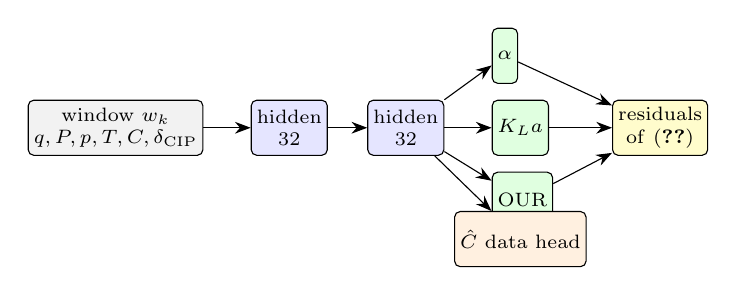
\begin{tikzpicture}[
  font=\scriptsize,
  box/.style={draw, rounded corners=2pt, align=center, minimum height=7mm, inner sep=2pt},
  arr/.style={-{Stealth[length=2mm]}}
]
\node[box, fill=gray!10] (in) {window $w_{k}$\\$q,P,p,T,C,\delta_{\mathrm{CIP}}$};
\node[box, fill=blue!10, right=6mm of in] (h1) {hidden\\32};
\node[box, fill=blue!10, right=5mm of h1] (h2) {hidden\\32};
\node[box, fill=green!12, above right=2mm and 6mm of h2] (a) {$\alpha$};
\node[box, fill=green!12, right=6mm of h2] (k) {$K_La$};
\node[box, fill=green!12, below right=2mm and 6mm of h2] (o) {OUR};
\node[box, fill=orange!12, below=7mm of k] (c) {$\hat{C}$ data head};
\node[box, fill=yellow!20, right=8mm of k] (res) {residuals\\of \eqref{eq:lphys}};
\draw[arr] (in) -- (h1);
\draw[arr] (h1) -- (h2);
\draw[arr] (h2) -- (a);
\draw[arr] (h2) -- (k);
\draw[arr] (h2) -- (o);
\draw[arr] (h2) -- (c);
\draw[arr] (a) -- (res);
\draw[arr] (k) -- (res);
\draw[arr] (o) -- (res);
\end{tikzpicture}
\caption{Soft-sensor heads. Only $\alpha$, $K_La$, and the oxygen uptake are published to the fan controller. The dissolved-oxygen head is a training target. The residual block is the physics constraint, not an extra measurement.}
\label{fig:pinn}
\end{figure}

\subsection{Identifiability}

The structural argument can be written as a sensitivity. From the curve residual, at fixed measured $q$ and $T$,
\begin{equation}
\label{eq:sens-kla}
\frac{\partial K_La}{\partial \alpha}
=
k_{\mathrm{ref}}
\left(\frac{q}{q_{\mathrm{ref}}}\right)^{0.82}
\theta^{\,T-20}
>
0.
\end{equation}
From the balance, at fixed $C$ and $\dot{C}$,
\begin{equation}
\label{eq:sens-our}
\frac{\partial\,\mathrm{OUR}}{\partial K_La}
=
\beta C^{*}(T)-C,
\end{equation}
which is nonzero whenever the tank is not saturated. The composition
\begin{equation}
\frac{\partial\,\mathrm{OUR}}{\partial \alpha}
=
\big(\beta C^{*}-C\big)
\frac{\partial K_La}{\partial \alpha}
\end{equation}
is therefore nonzero in every regime of Table~\ref{tab:regimes} at the set-points \eqref{eq:dosp}. A local change in $\alpha$ cannot hide inside the uptake. What can still go wrong is a slow trade along a flat valley of the loss if $q$ never moves and $\delta_{\mathrm{CIP}}$ never moves. The weekend mixing floor and the regime changes supply movement in $q$. The calendar supplies movement in $\delta_{\mathrm{CIP}}$. If a plant sits in one regime for many days, the sensor must hold $\alpha$ at its last healthy value rather than update it. The health bit implements that hold when the curvature of $\mathcal{L}_{\mathrm{phys}}$ with respect to $\alpha$, estimated by a finite difference on the window, falls below a small threshold. This is classical persistence of excitation, applied to one parameter \cite{ljung1999}.

A second ambiguity is probe bias. A probe that reads \SI{0.3}{\milli\gram\per\litre} low looks like a higher uptake. The fan-map residual does not see the probe, and the curve residual does not see it either. The balance does. The defense specified here is redundancy across time, not a second probe in the nominal design. Bias that is constant is absorbed by the controller's airflow bias \eqref{eq:bias} and does not require a correct $\alpha$. Bias that grows when $\delta_{\mathrm{CIP}}$ changes is indistinguishable from $\alpha$ without off-gas or a second probe. The specification therefore requires an off-gas or portable dissolved-oxygen check on a detergent day during commissioning, and it requires the health residual to be logged. It does not claim that the network detects every probe fault. A stuck probe that still produces a small balance residual, because the network has explained the stuck value with a ridiculous uptake, is caught by the bound on uptake rate of change, which is part of $\mathcal{L}_{\mathrm{bound}}$. If the uptake head moves faster than the kinetic ceiling $q_{\mathrm{COD}}X$ can justify, $h_{\mathrm{sensor}}$ is cleared.

\subsection{Handshake with the fan law}

The sensor publishes at the same one-minute clock as Algorithm~\ref{alg:deployed}. The message is $(\alpha, K_La, \mathrm{OUR}, h_{\mathrm{sensor}})$. The controller uses $\alpha$ in \eqref{eq:invert} and uses $\mathrm{OUR}$ as the measured uptake in that inversion. Publishing $K_La$ as well lets the controller check consistency:
\begin{equation}
\label{eq:consist}
\left|
\frac{K_La^{\mathrm{curve}}(\alpha,q,T)}{K_La}
-
1
\right|
\le
0.15.
\end{equation}
If \eqref{eq:consist} fails, $h_{\mathrm{sensor}}$ is treated as clear even if the sensor set it. The check is a tripwire against a software fault, not a second estimator. It is the sort of assertion an automation specification should contain and a machine-learning specification often forgets.

The lag of $0.30\,\mathrm{h}$ applied to $\alpha$ in the estimation is part of the sensor deployment, not part of the network. It is a filter
\begin{equation}
\label{eq:alpha-lag}
\dot{\alpha}_{\mathrm{used}}
=
\frac{1}{0.30}
\big(\alpha_{\mathrm{raw}}-\alpha_{\mathrm{used}}\big)
\end{equation}
that keeps a single noisy window from moving the fans. During the nominal week the raw value is the true regime $\alpha$, and the filter is what the controller sees. That choice makes the estimation a test of the information pattern and the lag, not a test of a particular random seed of a trained network. A trained network whose error is larger than this filtered truth will do worse. The estimation is therefore an upper bound on performance of the combined system, and Chapter~\ref{ch:estimate} says so in those words.

\subsection{Numerical illustration of the residual}

Take a quiet base point and a detergent point and evaluate the balance residual that training sees. At the base point of the hand inversion, $K_La=3.19\,\mathrm{h^{-1}}$, driving force \SI{5.64}{\milli\gram\per\litre}, transfer rate $3.19\times 5.64=18.0\,\mathrm{mg\,L^{-1}\,h^{-1}}$. If the uptake is also \SI{18}{\milli\gram\per\litre\per\hour} and $\dot{C}=0$, the first residual in \eqref{eq:lphys} is zero. At the detergent point, suppose the network keeps the old $\alpha=0.60$ while the true value is $0.40$. The curve then overstates $K_La$ by $0.60/0.40=1.5$. The predicted transfer rate is one and a half times the true rate. The residual is about half of the true uptake, which on the clean-in-place window is tens of milligrams per litre per hour, far above probe noise. The loss therefore has a reason to move $\alpha$ down, provided the detergent flag or the power measurement stops the network from instead inventing a matching drop in uptake. The curve residual is what stops that invention. This arithmetic is the reason the third term in \eqref{eq:lphys} is not optional.

\subsection{Failure modes the sensor must declare}

Three failures are specified, and each has a controller response that does not require a new optimization.

\begin{enumerate}[leftmargin=1.6em,itemsep=0.45em]
\item The health bit clears because the residual is large. The controller loads $\alpha$ from the regime table and continues. Energy optimality is weaker. The plant remains defined.
\item The probe is declared stuck by the uptake bound. The controller freezes $q$ at the last healthy value and raises an alarm. Freezing is safer than integrating \eqref{eq:bias} against a dead measurement. An operator can force the proportional-integral loop, which remains coded in the programmable controller.
\item The calendar feed is lost. $\sigma$ in \eqref{eq:scale} is set to $1$ and $C_{\mathrm{sp}}$ stays on the current regime. The sensor continues. The controller becomes the fixed-$\alpha$ predictive inversion if the sensor also fails, and it becomes a schedule-blind but $\alpha$-aware inversion if only the calendar fails. Those degradations are ordered on purpose. Losing $\alpha$ during detergent is more expensive than losing a preview of a load the probe will eventually see.
\end{enumerate}

Table~\ref{tab:degrade} collects the degradations. It is the interface specification between the two technologies. A design that only describes the healthy path has not finished the system.

\begin{table}[ht]
\centering
\caption{Degraded modes of the combined controller. Each row is reachable without changing code, by clearing a health bit.}
\label{tab:degrade}
\begin{tabular}{@{}p{3.4cm}p{4.2cm}p{5.4cm}@{}}
\toprule
Fault & $\alpha$ source & Preview \\
\midrule
None & soft sensor, lagged & calendar, $0.75\,\mathrm{h}$ \\
Sensor residual high & regime table & calendar kept \\
Probe stuck & last healthy $\alpha$ & airflow frozen \\
Calendar lost & soft sensor kept & $\sigma=1$, set-point held \\
Sensor and calendar lost & regime table of the last known regime & none; bias held \\
\bottomrule
\end{tabular}
\end{table}

\subsection{Relation to the estimation that follows}

Chapter~\ref{ch:estimate} integrates Algorithm~\ref{alg:deployed} on \eqref{eq:sb}--\eqref{eq:do-bal}, with $\alpha$ supplied by the lagged truth as the best case of \eqref{eq:alpha-lag}, and with the exhaust power \eqref{eq:exhaust} added after the integration. It also integrates three comparators that disable pieces of the same algorithm. Constant speed disables the inversion. The proportional-integral loop disables the inversion and the calendar and replaces them with \eqref{eq:pi} at $C_{\mathrm{sp}}=2.5\,\mathrm{mg/L}$. The fixed-$\alpha$ predictive inversion keeps \eqref{eq:invert} but locks $\alpha$ at $0.55$ and sets $\sigma=1$. The differences among those four integrals are the estimate of what the two technologies are worth on this train. They are not an estimate of what they are worth on a train with a different volume, a different diffuser, or a calendar the encoder has mis-labelled. The specification in this chapter is what would be re-run, not a universal percentage.

\section{Worked fan map, staging, and sensor cycle}
\label{sec:worked}

The specification in Section~\ref{sec:saempc} and Section~\ref{sec:piots} is executable only if a reader can reproduce a power, a staging, and a health decision from the formulae without opening the integrator. This section does those three calculations at the points the estimation later occupies, and it records the cycle time the edge computer must finish inside.

\subsection{Header power at the flows the week actually uses}

Equation~\eqref{eq:polytropic} with the numerical header \eqref{eq:dp-num} is evaluated here at six airflows. Inlet pressure is \SI{101.3}{\kilo\pascal}, inlet temperature is \SI{293.15}{\kelvin}, the specific gas constant of air is \SI{287}{\joule\per\kilogram\per\kelvin}, and the efficiency product is $0.70\times 0.95\times 0.97=0.645$. Mass flow uses \SI{1.293}{\kilogram\per\cubic\metre} at normal conditions, so $\dot{m}=1.293\,q/3600$ with $q$ in normal cubic metres per hour. The polytropic factor is
\begin{equation}
\label{eq:factor}
\Phi
=
\frac{\gamma}{\gamma-1}
\left[
\left(\frac{p_{\mathrm{in}}+\Delta p}{p_{\mathrm{in}}}\right)^{(\gamma-1)/\gamma}
-
1
\right]
=
3.5
\left[
r_{p}^{\,0.2857}
-
1
\right].
\end{equation}
Table~\ref{tab:powermap} is the result. The constant-speed flow of the estimation, \SI{6552}{\nmcph}, lands at \SI{185.5}{\kilo\watt}, which is why that loop averages \SI{185.4}{\kilo\watt} over a week that never changes speed. The hand inversion of the base regime, about \SI{1550}{\nmcph}, lands at \SI{32.6}{\kilo\watt}. One sentence in Section~\ref{sec:saempc} called that ``a few tens of kilowatts.'' The table is the sentence made numeric.

\begin{table}[ht]
\centering
\caption{Header pressure rise and electrical power from \eqref{eq:dp-num} and \eqref{eq:polytropic}. These rows are the fan model. They are not a catalogue curve.}
\label{tab:powermap}
\small
\begin{tabular}{@{}rrrrr@{}}
\toprule
$q$ (\si{\nmcph}) & $\Delta p$ (kPa) & pressure ratio & adiabatic kW & electrical kW \\
\midrule
900  & 52.4 & 1.518 & 12.1 & 18.7 \\
1550 & 53.3 & 1.526 & 21.1 & 32.6 \\
2500 & 55.4 & 1.547 & 35.1 & 54.4 \\
3500 & 58.7 & 1.580 & 51.7 & 80.1 \\
5200 & 66.9 & 1.660 & 85.7 & 132.9 \\
6552 & 75.6 & 1.746 & 119.7 & 185.5 \\
\bottomrule
\end{tabular}
\end{table}

Two features of the table are the reason the cube law was rejected for the blowers. From \SI{1550}{\nmcph} to \SI{3100}{\nmcph} a pure cube law, anchored at \SI{32.6}{\kilo\watt}, would predict $32.6\times 2^{3}=261\,\mathrm{kW}$. The header model at \SI{3500}{\nmcph} is only \SI{80}{\kilo\watt}, because most of the pressure is the static submergence, which does not grow with the square of speed. A controller tuned on the cube law would refuse legitimate airflow in the clean-in-place window, believing the power to be three times what the header actually draws. The exhaust fans are the opposite case, and they keep the cube law, because their pressure is duct pressure.

The surge arithmetic that goes with the table is short. Rated flow of one machine is \SI{2800}{\nmcph}. Surge at rated speed is $0.22\times 2800=616\,\mathrm{Nm^{3}/h}$. The margin of $1.15$ raises the floor to $708\,\mathrm{Nm^{3}/h}$. The plant mixing floor is \SI{900}{\nmcph} on one machine, which clears $708$. Two machines sharing \SI{900}{\nmcph} would each see \SI{450}{\nmcph}, which does not clear $708$. Equation~\eqref{eq:stage-rule} therefore keeps one machine online below \SI{2600}{\nmcph}. The boundary \SI{2600}{\nmcph} is not the surge number. It is a hysteresis choice: one machine at \SI{2600}{\nmcph} is below rated \SI{2800}{\nmcph}, and two machines at \SI{2600}{\nmcph} would each see \SI{1300}{\nmcph}, which clears surge at full speed and also at the reduced speed the fan law assigns to that flow. The rule is conservative on the low side and does not need an integer solver while the three machines are the same size.

\subsection{Staging at the three loads that matter}

Table~\ref{tab:stage} applies the rule to three header flows taken from the power map and from the shape of the week: quiet base, a mid load, and the constant-speed design point. Speed fraction is header flow divided by $n$ times rated flow, which is the right fraction only when the machines run at the flow the oxygen balance asked for and the header pressure is whatever \eqref{eq:dp-num} says. It is a check, not a second controller.

\begin{table}[ht]
\centering
\caption{Staging rule \eqref{eq:stage-rule} at three header flows. Per-machine flow is compared with the \SI{708}{\nmcph} surge margin at rated speed. At reduced speed the surge flow itself falls with \eqref{eq:fanlaws}, so the rated-speed comparison is the stricter one.}
\label{tab:stage}
\small
\begin{tabular}{@{}rrrrl@{}}
\toprule
Header $q$ & $n$ & $q$ each & speed fraction & surge check \\
\midrule
1550 & 1 & 1550 & 0.55 & clear of 708 \\
3500 & 2 & 1750 & 0.63 & clear of 708 \\
6552 & 3 & 2184 & 0.78 & clear of 708 \\
\bottomrule
\end{tabular}
\end{table}

The constant-speed point uses all three machines at a speed fraction of about $0.78$. That is a legal point. It is also an expensive point in every hour whose oxygen balance does not ask for it, which is most of the week. The proposed loop's base flow near \SI{1550}{\nmcph} uses one machine. The start of a second machine is then a real event, counted by $\lambda_{z}$ in \eqref{eq:p1}, and it happens when the calendar, not a noisy dissolved-oxygen error, says the load is coming. That is the operational content of hybrid control on this header \cite{bemporad1999hybrid,cristea2011}. A proportional-integral loop can start the second machine too, through a pressure or flow sequencer in the drive panel. It starts the machine after the error exists. The calendar starts it before the error exists. The estimation's dissolved-oxygen minima are the measurement of that difference.

\subsection{Clean-in-place inversion, continued}

The base inversion in Section~\ref{sec:saempc} is repeated here for the fermentation window so the two ends of the fan map are both hand-checked. Take an uptake of \SI{30}{\milli\gram\per\litre\per\hour}, which is the order of the feasible equilibrium discussed in Section~\ref{sec:problem}, a set-point of \SI{2.2}{\milli\gram\per\litre}, $T=\SI{33}{\celsius}$, and $\alpha=0.40$. Saturation at \SI{33}{\celsius} is \SI{7.16}{\milli\gram\per\litre}, so $\beta C^{*}=6.80$ and the driving force is $6.80-2.2=4.60$. Then
\begin{equation}
K_La^{\star}
=
30/4.60
=
6.52\,\mathrm{h^{-1}}.
\end{equation}
The temperature factor is $1.024^{13}$. Since $1.024^{10}\approx 1.268$ and $1.024^{3}\approx 1.074$, the product is about $1.36$. The denominator of the airflow ratio is
\begin{equation}
\alpha\,k_{\mathrm{ref}}\,\theta^{\,T-20}
=
0.40\times 6.5\times 1.36
=
3.54\,\mathrm{h^{-1}}.
\end{equation}
Hence $(q/2500)^{0.82}=6.52/3.54=1.84$, and
\begin{equation}
\frac{q}{2500}
=
1.84^{\,1/0.82}
=
1.84^{\,1.220}.
\end{equation}
Now $1.84^{1}=1.84$ and $1.84^{0.22}\approx 1.14$, so the product is about $2.10$ and $q\approx\SI{5250}{\nmcph}$. Table~\ref{tab:powermap} places \SI{5200}{\nmcph} at \SI{133}{\kilo\watt}. The staging rule turns on two machines below \SI{5200}{\nmcph} and the third at \SI{5200}{\nmcph} and above, so this point sits on the boundary and the implementation must apply the inequality in one direction only. Algorithm~\ref{alg:deployed} uses $n=3$ when $q\ge 5200$, which is the safe side of the boundary: three machines at \SI{1750}{\nmcph} each remain above the surge margin. The weekly integrator's fermentation-window mean power, about \SI{136}{\kilo\watt} for the proposed loop, is the same neighbourhood as this hand value. Agreement at that level is the implementation test. Agreement to the kilowatt would require the integrator's uptake to equal the \SI{30}{\milli\gram\per\litre\per\hour} assumed here, which it will not, because uptake moves with substrate.

If the same inversion is repeated with the quiet-week factor $\alpha=0.55$ instead of $0.40$, the denominator grows by $0.55/0.40=1.375$ and the airflow falls by $1.375^{1.220}\approx 1.47$. The controller that has not seen the detergent asks for about \SI{3570}{\nmcph} when the tank needs about \SI{5250}{\nmcph}. The bias \eqref{eq:bias} has to make up a factor of roughly $1.47$ by integrating a dissolved-oxygen error. With $K_{b}=0.55\,\mathrm{h^{-1}}$ that correction is a large fraction of an hour, which is the origin of the deeper dissolved-oxygen sag of the fixed-$\alpha$ loop. The arithmetic does not depend on the neural network. It depends on $\alpha$ being wrong by the amount Table~\ref{tab:regimes} states.

\subsection{Sensor cycle and health rule}

The soft sensor's training loss was specified in \eqref{eq:lphys}. The deployed cycle is a smaller object and should be written as its own procedure so it can be reviewed without the training code. Normalization is fixed from the commissioning week, not recomputed online, because an online mean would move when a detergent arrives and would hide the very shift the sensor is for. The scales used with this plant's units are: airflow divided by \SI{2500}{\nmcph}, power divided by \SI{80}{\kilo\watt}, header pressure minus \SI{52}{\kilo\pascal} then divided by \SI{20}{\kilo\pascal}, temperature minus \SI{30}{\celsius} then divided by $5$, dissolved oxygen divided by $3$, and the detergent flag left as $0$ or $1$. A window of thirty samples at one minute is concatenated and passed through the two hidden layers. The health decision does not trust the sigmoid. It trusts the residual.

\begin{algorithm}[ht]
\caption{One-minute sensor publish}
\label{alg:sensor}
\KwIn{window $w$, frozen weights $\phi$, curve \eqref{eq:kla-est}}
\KwOut{$\alpha$, $K_La$, $\mathrm{OUR}$, health bit}
Evaluate the four heads on $w$\;
Compute $\mathcal{L}_{\mathrm{phys}}$ on $w$ with \eqref{eq:lphys}\;
\eIf{uptake head changed faster than $q_{\mathrm{COD}}X$ over the window}{
  health $\leftarrow 0$\;
}{
  \eIf{emitted $\alpha\notin[0.15,0.90]$ or $\mathcal{L}_{\mathrm{phys}}>\epsilon$}{
    health $\leftarrow 0$\;
  }{
    health $\leftarrow 1$\;
  }
}
Publish the lagged $\alpha$ from \eqref{eq:alpha-lag} together with $K_La$ and $\mathrm{OUR}$\;
\end{algorithm}

The threshold $\epsilon$ is set during commissioning as a high quantile of $\mathcal{L}_{\mathrm{phys}}$ on a week that includes one real detergent day and that has been checked with a portable dissolved-oxygen probe or an off-gas hood \cite{leu2009,redmon1983,asce2007oxygen}. Setting $\epsilon$ on a quiet week only would mark every detergent day as a fault, and the controller would then ignore the sensor exactly when Table~\ref{tab:degrade} says the sensor is the point. Setting $\epsilon$ so large that the bit never clears removes the fallback. The quantile is the compromise, and it is a logged parameter, not a weight inside $\phi$.

Inference cost is small next to the minute. Two layers of $32$ units on a window of a few hundred inputs is well under a million floating-point operations. The edge computer's minute also contains the inversion \eqref{eq:invert}, which is a few dozen operations, and the log write. The minute is not tight. What is tight is the rule that a late publish is a missed publish. If Algorithm~\ref{alg:sensor} has not finished when Algorithm~\ref{alg:deployed} runs, the controller keeps the previous $\alpha$ and does not block the fan command on a network timeout. A fan command that waits for a learning model is a fan command that Level~1 should ignore.

\subsection{What the two algorithms guarantee together}

Taken as a pair, Algorithm~\ref{alg:deployed} and Algorithm~\ref{alg:sensor} guarantee the following on the model of Chapter~\ref{ch:previous}, and only on that model. The airflow command is always inside $[q_{\min},q_{\max}]$. The staging always puts each online machine at or above the surge margin used to write \eqref{eq:stage-rule}, because the rule's breakpoints were checked in Table~\ref{tab:stage} and the algorithm increases $n$ if the check fails. The bias cannot wind past $25\%$ of the inverted flow. If the sensor is unhealthy, $\alpha$ comes from the regime table, which for the fermentation recipe is $0.40$ and not the quiet-week $0.55$. If the probe is stuck, the airflow freezes. None of these guarantees is a statement about a different tank volume. They are the acceptance tests of this design, and Chapter~\ref{ch:estimate} is where the nominal week is asked whether the tests hold.

\section{Open-loop detergent step and the linearized fan problem}
\label{sec:openloop}

The week integral in Chapter~\ref{ch:estimate} closes the dissolved-oxygen loop, so the fans move as soon as the error appears. That closure hides the size of the mistake a wrong $\alpha$ makes before the loop has time to act. This section freezes the airflow on purpose, for less than one hour, so the oxygen balance can be read as an initial-value problem. It then linearizes the same balance, because a quadratic program is the form a solver-based implementation of \eqref{eq:p1} will actually code when the integer staging is fixed.

\subsection{Frozen airflow after the detergent arrives}

Take the fermentation conditions of the hand inversion: uptake held at \SI{30}{\milli\gram\per\litre\per\hour}, temperature \SI{33}{\celsius}, $\beta C^{*}=6.80\,\mathrm{mg/L}$, and $\alpha=0.40$. Two airflows are frozen. The first, \SI{3570}{\nmcph}, is what the inversion computes if it still believes $\alpha=0.55$. The second, \SI{5250}{\nmcph}, is the inversion at the true $\alpha$. The transfer coefficient follows \eqref{eq:kla-est}. Dissolved oxygen is integrated with the semi-implicit step \eqref{eq:semi} at $\Delta t=0.1\,\mathrm{h}$, starting from \SI{1.80}{\milli\gram\per\litre}. Uptake is not allowed to fall as dissolved oxygen falls. That is the conservative open-loop case: the biomass keeps asking for oxygen the fans are not delivering. In the closed-loop plant, uptake does fall, through $\mu_{C}$ in \eqref{eq:monod}, which is why a week minimum of \SI{0.90}{\milli\gram\per\litre} is not the same number as the open-loop end point below.

\begin{table}[ht]
\centering
\caption{Open-loop dissolved oxygen after a detergent step, uptake held at \SI{30}{\milli\gram\per\litre\per\hour}. The short column is the airflow a controller computes with $\alpha=0.55$. The corrected column uses $\alpha=0.40$.}
\label{tab:openloop}
\begin{tabular}{@{}ccc@{}}
\toprule
Time (h) & $C$ at \SI{3570}{\nmcph} & $C$ at \SI{5250}{\nmcph} \\
\midrule
0.0 & 1.80 & 1.80 \\
0.1 & 1.37 & 1.95 \\
0.2 & 1.08 & 2.05 \\
0.3 & 0.89 & 2.10 \\
0.4 & 0.75 & 2.14 \\
0.5 & 0.66 & 2.16 \\
0.6 & 0.60 & 2.17 \\
0.8 & 0.53 & 2.18 \\
\bottomrule
\end{tabular}
\end{table}

At the wrong airflow the transfer coefficient is $4.74\,\mathrm{h^{-1}}$. Oxygen transfer at the initial dissolved oxygen is $4.74\times(6.80-1.80)=23.7\,\mathrm{mg\,L^{-1}\,h^{-1}}$, against an uptake of $30$, so the tank loses oxygen at about \SI{6}{\milli\gram\per\litre\per\hour} immediately and faster as the driving force grows. By $0.3\,\mathrm{h}$ the open-loop concentration is already under \SI{1}{\milli\gram\per\litre}. At the corrected airflow the coefficient is $6.50\,\mathrm{h^{-1}}$, transfer at the initial state is $6.50\times 5.00=32.5$, slightly above the uptake, and the concentration climbs to the set-point neighbourhood of \SI{2.2}{\milli\gram\per\litre} and stops. The two columns are the same balance. The only change is whether $\alpha$ in the inversion is the quiet-week number or the detergent number. That is the entire content of the second technology, seen without a neural network and without a week of feedback: forty-five minutes of believing the wrong factor is enough, in open loop, to cross the operational floor.

Feedback reduces the damage, and the estimation shows how much. The fixed-$\alpha$ loop in Table~\ref{tab:do-cip} reaches a minimum of \SI{0.90}{\milli\gram\per\litre}, not \SI{0.53}{\milli\gram\per\litre}, because the bias \eqref{eq:bias} adds air as soon as the probe falls, and because uptake itself declines when $\mu_{C}$ declines. The proposed loop, which does not wait for the probe, stays at a minimum of \SI{1.63}{\milli\gram\per\litre}. Table~\ref{tab:openloop} is the reason that difference exists. It is not a second estimate of the week.

\subsection{Linear model used when staging is held}

Between staging events $n$ is constant and $q$ is the only continuous input. Linearize \eqref{eq:do-bal} at an equilibrium $(C_{0},q_{0},\alpha_{0})$ where transfer equals uptake. With $K_La$ from \eqref{eq:kla-est},
\begin{equation}
\label{eq:klin}
\frac{\partial K_La}{\partial q}
=
0.82\,
\frac{K_La}{q},
\qquad
\frac{\partial K_La}{\partial \alpha}
=
\frac{K_La}{\alpha}.
\end{equation}
The dissolved-oxygen deviation $c=C-C_{0}$ then obeys
\begin{equation}
\label{eq:clin}
\dot{c}
=
-a\,c
+
b_{q}\,\delta q
+
b_{\alpha}\,\delta\alpha
-
\delta\mathrm{OUR},
\end{equation}
where
\begin{align}
a
&=
K_La(q_{0},\alpha_{0}),
\\
b_{q}
&=
0.82\,
\frac{K_La}{q_{0}}
\big(\beta C^{*}-C_{0}\big),
\\
b_{\alpha}
&=
\frac{K_La}{\alpha_{0}}
\big(\beta C^{*}-C_{0}\big).
\end{align}
The pole $-a$ is the transfer coefficient itself. At the base hand inversion, $a\approx 3.2\,\mathrm{h^{-1}}$, so the open-loop time constant of dissolved oxygen is about twenty minutes. A preview of $0.75\,\mathrm{h}$ is a little more than two time constants. A preview of one minute is not a preview. This is the quantitative link between the blower lag of $0.10\,\mathrm{h}$, the oxygen time constant, and the calendar lead specified in Section~\ref{sec:saempc}.

At the corrected detergent point, $q_{0}=5250$, $K_La=6.50$, $C_{0}=2.2$, $\alpha_{0}=0.40$, the driving force is $4.60$, and
\begin{equation}
b_{q}
=
0.82\times
\frac{6.50}{5250}
\times
4.60
=
0.00467
\quad
\mathrm{mg\,L^{-1}\,h^{-1}}
\text{ per }
\mathrm{Nm^{3}/h}.
\end{equation}
An extra \SI{200}{\nmcph} therefore adds about \SI{0.93}{\milli\gram\per\litre\per\hour} of transfer at that point, before the concentration has moved. The same increment at the wrong-$\alpha$ airflow is not the right correction: the plant needs on the order of \SI{1700}{\nmcph} more air, which is outside the linear range of a model built at \SI{3570}{\nmcph}. The linear model is for the tracking layer once $\alpha$ is right. It is not a substitute for putting the right $\alpha$ in the inversion. That distinction keeps the quadratic program honest. It optimizes deviations. It does not discover the detergent.

Discretize \eqref{eq:clin} at the one-minute controller step $\Delta t=1/60\,\mathrm{h}$ with a zero-order hold on $\delta q$. The exact discrete step for a scalar pole is
\begin{equation}
\label{eq:cdisc}
c_{k+1}
=
e^{-a\Delta t}\,c_{k}
+
\frac{1-e^{-a\Delta t}}{a}
\big(
b_{q}\,\delta q_{k}
+
b_{\alpha}\,\delta\alpha_{k}
-
\delta\mathrm{OUR}_{k}
\big).
\end{equation}
With $a=6.50\,\mathrm{h^{-1}}$ and $\Delta t=1/60$, $a\Delta t=0.108$ and $e^{-a\Delta t}\approx 0.897$. About ten percent of a concentration error is forgotten each minute if the input is held at the equilibrium airflow. A bias that adds airflow every minute is therefore fast enough to remove a small offset and too slow, as Table~\ref{tab:openloop} shows, to remove a forty-percent error in $\alpha$ before the floor is crossed. Equation~\eqref{eq:cdisc} is what a tracking quadratic program should embed. The economic hinges \eqref{eq:hinge-c} and \eqref{eq:hinge-s} remain outside the quadratic part, as linear slacks, which is the standard transcription \cite{rawlings2017mpc,boyd2004convex,maciejowski2002}.

\subsection{Slack form of the economic problem at fixed staging}

With $n$ fixed, the decision at each step of a horizon of $N$ minutes is $\delta q_{k}$ and two non-negative slacks $s^{C}_{k}$ and $s^{S}_{k}$. Power is replaced by its tangent at $q_{0}$,
\begin{equation}
\label{eq:ptan}
P(q_{0}+\delta q)
\approx
P(q_{0})
+
P'(q_{0})\,\delta q,
\end{equation}
and $P'$ is read off Table~\ref{tab:powermap} rather than off a cube law. Between \SI{1550}{\nmcph} and \SI{2500}{\nmcph} the secant is $(54.4-32.6)/(2500-1550)=0.0229\,\mathrm{kW}$ per $\mathrm{Nm^{3}/h}$. Between \SI{5200}{\nmcph} and \SI{6552}{\nmcph} the secant is $(185.5-132.9)/(6552-5200)=0.0389\,\mathrm{kW}$ per $\mathrm{Nm^{3}/h}$. The slope rises, but it does not triple. A quadratic program that used $P\propto q^{3}$ would put a much steeper price on the detergent airflow and would talk the optimizer out of the air Table~\ref{tab:openloop} shows is necessary.

The slack problem at fixed $n$ is then
\begin{equation}
\label{eq:qp}
\begin{aligned}
\min_{\delta q,\,s}
\quad
&
\sum_{k=0}^{N-1}
\left(
P'(q_{0})\,\delta q_{k}\,\Delta t
+
\lambda_{C}\,s^{C}_{k}
+
\lambda_{S}\,s^{S}_{k}
\right)
\\
\text{subject to}\quad
&
\eqref{eq:cdisc},
\\
&
C_{0}+c_{k}+s^{C}_{k}
\ge
C_{\mathrm{floor}},
\\
&
s^{C}_{k}\ge 0,
\quad
s^{S}_{k}\ge 0,
\\
&
q_{\min}
\le
q_{0}+\delta q_{k}
\le
q_{\max}^{(n)},
\end{aligned}
\end{equation}
where $q_{\max}^{(n)}$ is the largest header flow the online machines can deliver without crossing the motor limit, and the chemical-oxygen-demand slack is supplied by a similar linearization of \eqref{eq:sb} that this paragraph does not repeat. The program \eqref{eq:qp} is convex. It can be solved by any interior-point code already cited for the nonlinear case \cite{wachter2006ipopt,nocedal2006,boyd2004convex}. It does not choose $n$. The integer rule, or an enumeration over $n\in\{1,2,3\}$ of three convex programs, chooses $n$. Three convex programs per minute is a trivial load. It is also the clean way to upgrade Algorithm~\ref{alg:deployed} when the machines stop being identical: replace the rule by the enumeration, and keep the same slacks.

Move blocking keeps the program small. Hold $\delta q$ constant over blocks of five minutes inside a horizon of sixty minutes, except for the first block, which is one minute so the command that is actually applied is free. The decision count is then about a dozen continuous moves plus slacks, not sixty. Nothing in the oxygen time constant argues for a new airflow every minute once the first move has been made. The one-minute publish remains, because the first block is re-optimized every minute in the usual receding-horizon way \cite{mayne2000mpc,qin2003mpc}.

\subsection{Where the soft sensor enters the linear problem}

In \eqref{eq:clin} the term $b_{\alpha}\,\delta\alpha$ is a measured disturbance if the sensor is healthy and a forecast error if it is not. A healthy sensor sets $\delta\alpha$ from the difference between the emitted $\alpha$ and the $\alpha_{0}$ at which the linear model was built, and the quadratic program treats that difference as known over the horizon, constant until the calendar says the recipe changes. An unhealthy sensor sets $\delta\alpha=0$ and relies on the slack $s^{C}$ and on the bias \eqref{eq:bias}. The program does not estimate $\alpha$. Estimation stays in Algorithm~\ref{alg:sensor}, where the residual \eqref{eq:lphys} has the nonlinear curve. Splitting the jobs this way is what makes the quadratic program convex and the sensor free to be nonlinear. Putting a neural network inside \eqref{eq:qp} would give up both properties for a coupling the plant does not need at a one-minute clock.

The numerical size of $b_{\alpha}$ at the detergent point is
\begin{equation}
b_{\alpha}
=
\frac{6.50}{0.40}\times 4.60
=
74.8
\quad
\mathrm{mg\,L^{-1}\,h^{-1}}
\text{ per unit $\alpha$}.
\end{equation}
A mistake of $0.15$ in $\alpha$, which is the gap between $0.55$ and $0.40$, is a transfer error of $74.8\times 0.15=11.2\,\mathrm{mg\,L^{-1}\,h^{-1}}$. Against an uptake of \SI{30}{\milli\gram\per\litre\per\hour} that is more than a third of the oxygen budget. No reasonable weight $\lambda_{C}$ will prefer to absorb a third of the budget in the slack if the sensor can remove it. The weight is for probe noise and for the minutes the filter \eqref{eq:alpha-lag} has not yet moved. It is not for a detergent hour lived at the wrong factor.

This section closes the specification. The week in Chapter~\ref{ch:estimate} uses the inversion form, not \eqref{eq:qp}, and the text there says so. The linear program is the upgrade path that keeps the same $\alpha$, the same calendar, the same floors, and the same fan map, and that replaces a one-step inversion with a horizon once the staging machines are no longer twins. The open-loop table is the reason the upgrade is not allowed to drop the sensor in order to simplify the program.

\subsection{One blocked hour, written out}

A sixty-minute horizon with five-minute blocks after a free first minute has one free move and eleven blocked moves if the first block is one minute and the rest are five, because $1+11\times 5=56$, and the last four minutes are held with the last block. The exact partition is not important. The pattern is. Denote the applied command by $q_{0}$ and the blocked commands by $q^{(1)},\ldots,q^{(11)}$. The concentration at minute $k$ depends on $q_{0}$ for every $k\ge 1$ and on block $b$ only for minutes inside and after that block. With the scalar transition $\Phi=e^{-a\Delta t}\approx 0.897$ at the detergent pole, the gain from a move that begins at minute $m$ to the concentration at minute $k>m$ is
\begin{equation}
\label{eq:gain}
g(k,m)
=
\frac{1-\Phi}{a}\,
b_{q}\,
\sum_{j=m}^{k-1}
\Phi^{\,k-1-j}.
\end{equation}
The inner sum is a geometric series,
\begin{equation}
\sum_{j=0}^{k-m-1}\Phi^{j}
=
\frac{1-\Phi^{\,k-m}}{1-\Phi},
\end{equation}
so
\begin{equation}
\label{eq:gain2}
g(k,m)
=
\frac{b_{q}}{a}
\left(
1-\Phi^{\,k-m}
\right).
\end{equation}
At the detergent point $b_{q}/a=0.00467/6.50=7.18\times 10^{-4}\,\mathrm{mg\,L^{-1}}$ per $\mathrm{Nm^{3}/h}$. A move of \SI{200}{\nmcph} that has been in force for many time constants changes dissolved oxygen by $200\times 7.18\times 10^{-4}=0.144\,\mathrm{mg/L}$. The same move, one minute old, has $\Phi^{1}\approx 0.90$, so $1-\Phi\approx 0.10$ and the change is only about $0.014\,\mathrm{mg/L}$. Most of the effect of an airflow decision is not visible in the probe at the next sample. A controller that retunes from the one-minute error alone, which is what a high-gain proportional term does, chases a signal that has not yet arrived. The integral term and the calendar exist because of \eqref{eq:gain2}. The calendar moves the airflow before minute $m$. The gain formula says the probe will agree about twenty minutes later, which is $1/a$ at this pole.

The power price of that early move is the secant from Table~\ref{tab:powermap}. At the detergent end of the map, $0.0389\,\mathrm{kW}$ per $\mathrm{Nm^{3}/h}$. Raising the header by \SI{1700}{\nmcph}, which is the gap between \SI{3570}{\nmcph} and \SI{5250}{\nmcph}, costs about $1700\times 0.0389=66\,\mathrm{kW}$ while the higher flow is held. Over the eighteen hours of the fermentation window that would be about $1200\,\mathrm{kWh}$ if the gap were held the entire time. The week does not hold it the entire time. The fixed-$\alpha$ loop spends $2186\,\mathrm{kWh}$ in the window and the proposed loop spends $2441\,\mathrm{kWh}$. The difference, $255\,\mathrm{kWh}$, is what a partial and delayed correction costs relative to arriving with the right airflow. It is much smaller than $1200\,\mathrm{kWh}$ because the bias does eventually add air, and it is large enough to buy the dissolved-oxygen minimum back from $0.90$ to $1.63\,\mathrm{mg/L}$. Equation~\eqref{eq:gain2} and that $255\,\mathrm{kWh}$ are the same fact at two scales: air that arrives before the concentration has moved is cheaper, in constraint violations, than air that arrives after.

The blocked horizon uses this by letting $q_{0}$ jump when the calendar flips $\delta_{\mathrm{CIP}}$, and by letting the later blocks sit on the new airflow rather than ramp in ignorance. A block that is not allowed to change until the probe has confirmed the detergent has the same defect as the proportional-integral loop, only with a solver in front of it. The solver is not the technology. The disturbance model inside the solver is the technology. On this plant the disturbance model is the recipe clock plus $\alpha$ from the residual \eqref{eq:lphys}. Remove either one and \eqref{eq:qp} is a competent tracking problem of a kind the literature already contains \cite{holenda2008,shen2008,zeng2015empc,cristea2011}. Keep both and the problem is the one stated in Chapter~\ref{ch:previous}.

\subsection{What the edge computer must log in that hour}

The blocked hour is also an audit object. For each publish the log line has to be reconstructible from the formulae, otherwise a later disagreement with the meter cannot be assigned to a cause. The minimum line is: time, regime identifier, detergent flag, $\alpha$ used and whether it came from the sensor or the table, health bit, dissolved-oxygen measurement, set-point, load scale $\sigma$, inverted airflow before the bias, bias, commanded airflow, staging $n$, and a saturation bit if the command met $q_{\min}$ or $q_{\max}$. That is fourteen fields. None of them is a weight inside a network. An operator can read $\sigma>1$ together with a detergent flag and know the calendar, not the probe, asked for air. An operator can read a cleared health bit and know the table value was substituted. The estimation in Chapter~\ref{ch:estimate} is a week of those lines, reduced to regime sums. A site that logs only dissolved oxygen and power can still compute kilowatt-hours. It cannot tell a calendar failure from a sensor failure from a drive limit, which are the three degradations in Table~\ref{tab:degrade}. The fourteen fields are therefore part of the fan controller, in the same sense that the surge inequality is part of it. A controller that cannot explain its last hour is not finished, however small its tracking error is on a benchmark file \cite{qin2003mpc,obrien2011,iratni2019,corominas2018}.

\chapter{System Build and Estimation}
\label{ch:estimate}

The specification in Chapter~\ref{ch:method} is not yet a plant. This chapter places it in an automation architecture and then estimates its behaviour by integrating the model of Section~\ref{sec:problem} over the week of Table~\ref{tab:regimes}. The architecture is buildable with equipment that a brewery treatment room already uses: a programmable controller for interlocks and inner loops, drives on the fans, a historian, and an edge computer for the minute-scale law and the soft sensor. The estimate is a simulation of that representative train. Absolute kilowatt-hours belong to the parameter set written in Chapter~\ref{ch:previous}. The comparisons belong to the information each controller is allowed to use.

\section{System build}
\label{sec:build}

\subsection{What is being built}

The build covers the cleaning plant from the inlet screen to the discharge flume. Production equipment upstream is not modified. The only production interface is a read of the batch and clean-in-place schedule. Figure~\ref{fig:train} is the process line the control system is drawn against. Liquid flows left to right. Air is a second network, drawn under the tanks that need it. The optimizer of Chapter~\ref{ch:method} writes set-points into this line. It does not replace the line.

\begin{figure}[ht]
\centering
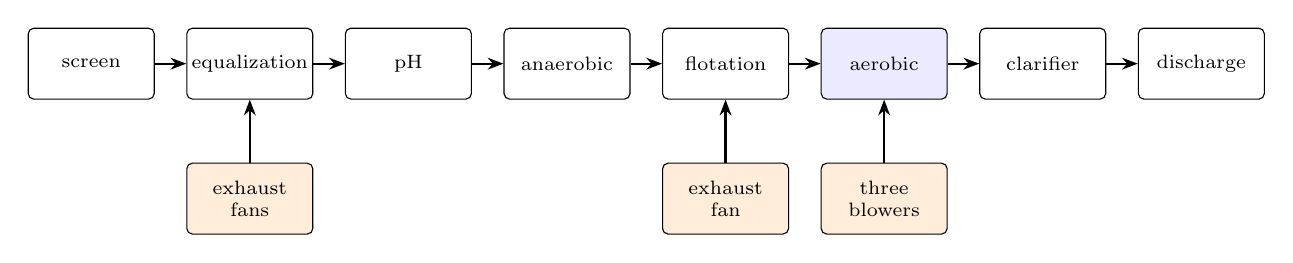
\begin{tikzpicture}[
  font=\scriptsize,
  unit/.style={draw, rounded corners=2pt, minimum width=16mm, minimum height=9mm, align=center, inner sep=1pt},
  arr/.style={-{Stealth[length=2mm]}, thick}
]
\node[unit] (sc) {screen};
\node[unit, right=4mm of sc] (eq) {equalization};
\node[unit, right=4mm of eq] (ph) {pH};
\node[unit, right=4mm of ph] (an) {anaerobic};
\node[unit, right=4mm of an] (daf) {flotation};
\node[unit, right=4mm of daf, fill=blue!8] (ae) {aerobic};
\node[unit, right=4mm of ae] (cl) {clarifier};
\node[unit, right=4mm of cl] (out) {discharge};
\draw[arr] (sc) -- (eq);
\draw[arr] (eq) -- (ph);
\draw[arr] (ph) -- (an);
\draw[arr] (an) -- (daf);
\draw[arr] (daf) -- (ae);
\draw[arr] (ae) -- (cl);
\draw[arr] (cl) -- (out);
\node[unit, fill=orange!15, below=8mm of eq] (ex1) {exhaust\\fans};
\node[unit, fill=orange!15, below=8mm of daf] (ex2) {exhaust\\fan};
\node[unit, fill=orange!15, below=8mm of ae] (bl) {three\\blowers};
\draw[arr] (ex1) -- (eq);
\draw[arr] (ex2) -- (daf);
\draw[arr] (bl) -- (ae);
\end{tikzpicture}
\caption{Cleaning train. Shaded units are the fan duties. Anaerobic pretreatment is in the train so the aerobic fans see a polishing load rather than raw brewery waste.}
\label{fig:train}
\end{figure}

Levels of control follow the enterprise-control split \cite{isa95}. Level 0 is the drives, valves, and sensors. Level 1 is the programmable controller, programmed in the languages of IEC 61131-3, and it is the only level that may drop a run command or open a contactor \cite{iec61131}. Level 2 is the edge computer that runs Algorithm~\ref{alg:deployed} and the soft sensor. Level 3 is the historian and the schedule import. The optimizer is not Level 1. If the edge computer stops, Level 1 continues on the proportional-integral loop with the last legal set-point, and it is required to do so without a download. That fallback is the difference between an optimization project and an operable plant \cite{obrien2011,olsson2012ica,iratni2019}.

\begin{figure}[ht]
\centering
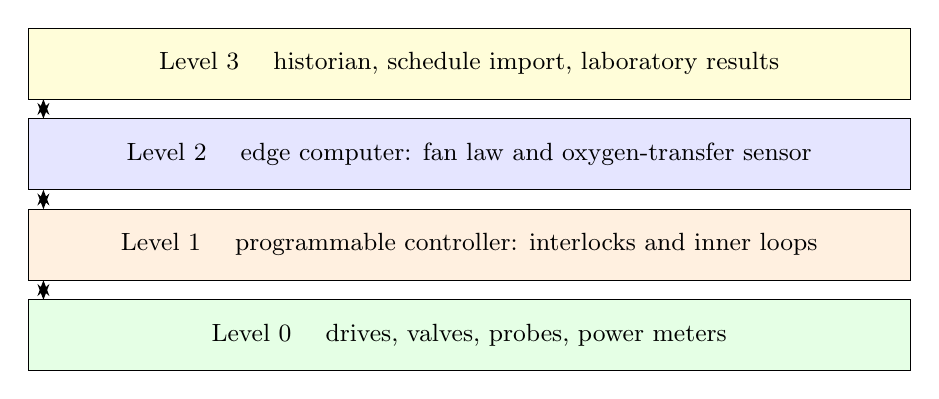
\begin{tikzpicture}[
  font=\small,
  layer/.style={draw, minimum width=11.2cm, minimum height=9mm, align=center, anchor=west},
  arr/.style={{Stealth[length=2mm]}-{Stealth[length=2mm]}, thick}
]
\node[layer, fill=yellow!15] (l3) at (0,0) {Level 3 \quad historian, schedule import, laboratory results};
\node[layer, fill=blue!10] (l2) at (0,-1.15) {Level 2 \quad edge computer: fan law and oxygen-transfer sensor};
\node[layer, fill=orange!12] (l1) at (0,-2.3) {Level 1 \quad programmable controller: interlocks and inner loops};
\node[layer, fill=green!10] (l0) at (0,-3.45) {Level 0 \quad drives, valves, probes, power meters};
\draw[arr] (0.2,-0.45) -- (0.2,-0.7);
\draw[arr] (0.2,-1.6) -- (0.2,-1.85);
\draw[arr] (0.2,-2.75) -- (0.2,-3.0);
\end{tikzpicture}
\caption{Control levels. Set-points move downward. Health bits and measurements move upward. Only Level 1 energizes a fan.}
\label{fig:levels}
\end{figure}

\subsection{Signals}

Table~\ref{tab:io} is the signal list the two technologies add to a plant that already has level, pH, and on--off control. It is not a full input-output schedule of the treatment works. It is the list without which Algorithm~\ref{alg:deployed} and the residual \eqref{eq:lphys} cannot be computed. Power meters are included on purpose. A fan law that trusts a commanded speed and never reads power cannot evaluate the middle residual of \eqref{eq:lphys}, and it cannot detect a machine that is on the schedule and off the shaft.

\begin{table}[ht]
\centering
\caption{Signals added for the fan optimizer and the transfer sensor. Scan times are Level~1 scan or faster. The edge computer subscribes at one-minute averages.}
\label{tab:io}
\begin{tabular}{@{}p{4.6cm}p{2.4cm}p{6.0cm}@{}}
\toprule
Signal & Direction & Use \\
\midrule
Delivered airflow, header & in & Inversion \eqref{eq:invert}, surge check, $K_La$ curve \\
Header pressure & in & Consistency with \eqref{eq:dp-num} \\
Blower power, each machine & in & Map residual, energy account \\
Blower speed, each machine & in & Surge law \eqref{eq:surge} \\
Blower run command & out & Staging word from Level 2, gated by Level 1 \\
Dissolved oxygen, aerobic & in & Bias \eqref{eq:bias}, balance residual \\
Temperature, aerobic & in & Saturation and $\theta$ correction \\
Influent flow and regime flag & in & Load scale $\sigma$, sensor window \\
Exhaust-fan speed, two rooms & out & Calendar fraction $\nu(\rho)$ in \eqref{eq:exhaust} \\
Schedule message & in & Preview $D$, detergent flag \\
Sensor health bit & internal & Fusion rule \eqref{eq:alpha-fuse} \\
\bottomrule
\end{tabular}
\end{table}

Communication from Level 1 to Level 2 is an OPC Unified Architecture session on the plant network, with the schedule message as a separate subscription from the production historian \cite{mahnke2009opc,isa95}. The edge computer does not sit on the drive network. A failure of the optimizer must not be a failure of the drive bus. Time synchronization is required only to a second. The lags in the plant are tenths of an hour. A one-second clock error is invisible next to the $0.75\,\mathrm{h}$ preview.

\subsection{Interlocks that override the optimizer}

The programmable controller enforces the following regardless of the set-point it has just received. A blower may not start if its outlet valve is shut. A blower that reports a drive fault is removed from the staging count and the edge computer is told the new $n_{\max}$. Header pressure above a mechanical trip stops all but one machine and opens a blow-off. Dissolved oxygen below \SI{0.4}{\milli\gram\per\litre} for more than ten minutes forces $n$ upward if a machine is available, even if the optimizer is silent. The exhaust fans run if their tank level is above the low-low cutout. None of these rules is an optimization. They are the reason Level 1 exists. The estimation below does not need to hit them on the nominal week. The build is incomplete if they are only in a manual.

Motor efficiency class is part of the build and not part of the control law. Machines on a variable-speed aeration duty should be specified to the current efficiency class for converter-fed motors, and the fan curve should be the tested curve, not a catalogue cube law \cite{iec60034,amca210,dixon2014turbo}. The power model \eqref{eq:polytropic} then uses the tested efficiency inside $\eta$. In the estimation, $\eta$ is the constant product $0.70\times 0.95\times 0.97$. A site curve would replace that product and would be read by the same residual.

\subsection{Software cycle}

The edge cycle is one minute, aligned to the historian. Inside the minute the sequence is fixed. Read averages. Update the $\alpha$ filter \eqref{eq:alpha-lag}. Evaluate the sensor residual on the last window and set the health bit. Run Algorithm~\ref{alg:deployed}. Publish $q$, $n$, and $\nu$. Log the residual, the health bit, the load scale, and the active degradation row of Table~\ref{tab:degrade}. Logging the degradation row is what makes a later audit possible. A plant that only logs dissolved oxygen cannot explain a week in which the calendar feed was down.

The proportional-integral fallback is tuned once, stored in the programmable controller, and not retuned by the edge computer. Its set-point is \SI{2.5}{\milli\gram\per\litre}, its proportional gain on airflow is $1400\,\mathrm{Nm^{3}\,h^{-1}}$ per $\mathrm{mg/L}$, and its integral gain is $500\,\mathrm{Nm^{3}\,h^{-1}}$ per $\mathrm{mg/L}$ per hour, with the integrator clamped at $\pm 8\,\mathrm{mg\,h\,L^{-1}}$ in the units of the implemented sum. Those are the gains of the baseline in Section~\ref{sec:est}, so the fallback the plant will actually run is the fallback the estimate measures. Gains that exist only in a paper and not in the controller image are not part of the build.

\subsection{Model used for the estimate}

The plant integrated in the estimate is exactly \eqref{eq:monod}--\eqref{eq:dp-num}, with the lags stated in Section~\ref{sec:problem}. The dissolved-oxygen update is semi-implicit,
\begin{equation}
\label{eq:semi}
C^{+}
=
\frac{
C
+
\Delta t\,
\big(
K_La\,\beta C^{*}
-
\mathrm{OUR}
\big)
}{
1
+
\Delta t\,
K_La
},
\end{equation}
which is the exact step of a linear transfer term and does not ring when $K_La$ is large. Substrate and ammonia use forward Euler with $\Delta t=0.02\,\mathrm{h}$. The controller is evaluated on the same grid and held between its own decisions. Four closed loops are integrated for $168\,\mathrm{h}$ from the same initial state ($S_{b}=40$, $S_{i}=30$, $S_{n}=4$, $C=2$, all in $\mathrm{mg/L}$).

The four loops are:

\begin{enumerate}[leftmargin=1.6em,itemsep=0.35em]
\item \textbf{Proposed.} Algorithm~\ref{alg:deployed}, lagged true $\alpha$ as the best case of the soft sensor, calendar preview of $0.75\,\mathrm{h}$, set-points \eqref{eq:dosp}.
\item \textbf{Proportional-integral.} The fallback gains above, fixed set-point \SI{2.5}{\milli\gram\per\litre}, no calendar, no $\alpha$.
\item \textbf{Fixed-$\alpha$ inversion.} Equation~\eqref{eq:invert} with $\alpha$ locked at $0.55$, load scale $\sigma=1$, set-point \SI{2.0}{\milli\gram\per\litre}, and the same bias filter. This is predictive control without either technology.
\item \textbf{Constant speed.} Airflow fixed at $1.15$ times the inversion of the fermentation clean-in-place equilibrium uptake at $\alpha=0.40$ and $C=\SI{2.2}{\milli\gram\per\litre}$, which evaluates to \SI{6552}{\nmcph}. The machine runs at that flow all week.
\end{enumerate}

Constant speed is the policy a plant uses when the drives are installed and nobody trusts a loop, or when the loop is in manual at the worst-hour valve position. It is the right first baseline. The proportional-integral loop is the right second baseline, because it is what Level 1 already contains. The fixed-$\alpha$ inversion separates the value of prediction from the value of $\alpha$ and the calendar.

The soft sensor in the proposed loop is not a freshly trained network with a random residual. It is the lagged true $\alpha$, filtered by \eqref{eq:alpha-lag}, with a two-percent caution. Chapter~\ref{ch:method} already called this an upper bound. The estimate therefore answers the question ``what is the information worth if the sensor is good,'' and not the question ``what residual will a particular training run leave.'' A commissioning test against off-gas is still required before the upper bound is treated as a site forecast \cite{leu2009,redmon1983}.

\section{Estimation}
\label{sec:est}

\subsection{Week totals}

Table~\ref{tab:week} gives the blower electricity and the discharge result for the four loops. Chemical oxygen demand violation hours count the time the aerobic effluent $S_{b}+S_{i}$ exceeds \SI{125}{\milli\gram\per\litre}. On this week, with this volume and this permit, every loop records zero violation hours. That fact is the first result and it should not be rounded into a claim of superior compliance. The tank and the kinetic ceiling can meet the study limit even when dissolved oxygen sags, provided the sag is not held for a long time near zero. The loops separate on energy and on how close they come to the dissolved-oxygen floor, not on a violation count that is zero for all of them.

\begin{table}[ht]
\centering
\caption{Blower electricity and discharge over the representative week. Violation hours are time above \SI{125}{\milli\gram\per\litre} chemical oxygen demand. The last column is energy divided by the constant-speed energy.}
\label{tab:week}
\small
\begin{tabular}{@{}lrrrr@{}}
\toprule
Loop & kWh & Mean kW & Viol.\ (h) & Fraction of constant speed \\
\midrule
Proposed & 9656 & 57.5 & 0 & 0.31 \\
Fixed-$\alpha$ inversion & 9620 & 57.3 & 0 & 0.31 \\
Proportional-integral & 10920 & 65.0 & 0 & 0.35 \\
Constant speed & 31151 & 185.4 & 0 & 1 \\
\bottomrule
\end{tabular}
\end{table}

Against constant speed, the proposed loop uses $31151-9656=21495\,\mathrm{kWh}$ less in the week, which is $69.0\%$. Against the proportional-integral fallback, it uses $10920-9656=1264\,\mathrm{kWh}$ less, which is $11.6\%$. Against the fixed-$\alpha$ inversion it uses $36\,\mathrm{kWh}$ more, about $0.4\%$. The last comparison is the interesting one. A predictive inversion that holds a sensible set-point already captures almost all of the energy. What the schedule and the live $\alpha$ buy on this week is not another large energy cut. They buy dissolved-oxygen margin during the detergent window, which the next table shows, and they buy a controller that does not depend on an operator having chosen \SI{2.0}{\milli\gram\per\litre} in advance. The proportional-integral loop holds \SI{2.5}{\milli\gram\per\litre} because that is the operator habit encoded in the fallback. The economic set-points \eqref{eq:dosp} are lower in the quiet hours and are the main reason the proposed loop beats the fallback on energy.

At an illustrative price of $0.12$ currency units per kilowatt-hour, used only as a conversion and not as a tariff study, the week is worth about $152$ currency units against the proportional-integral loop and about $2580$ currency units against constant speed. Over fifty-two such weeks the constant-speed gap is of order $1.3\times 10^{5}$ currency units a year on blower electricity alone. The number scales with the price and with how often the plant actually sits at the worst-hour valve. It does not scale the physics.

Flow over the week is
\begin{equation}
\begin{aligned}
&50\times 96
+
70\times 30
+
75\times 18
+
68\times 12
+
22\times 12
\\
&\quad
=
4800+2100+1350+816+264
=
9330\,\mathrm{m^{3}}.
\end{aligned}
\end{equation}
Specific blower energy of the proposed loop is $9656/9330=1.03\,\mathrm{kWh/m^{3}}$. The proportional-integral loop is $1.17\,\mathrm{kWh/m^{3}}$. Constant speed is $3.34\,\mathrm{kWh/m^{3}}$. Chemical oxygen demand mass fed to the aerobic tank is $3747\,\mathrm{kg}$ in the week, so the proposed loop uses $2.58\,\mathrm{kWh}$ per kilogram of aerobic influent chemical oxygen demand. These normalizations are arithmetic on Table~\ref{tab:regimes} and Table~\ref{tab:week}. They are the right way to carry the result to a plant with a different weekly volume, and they are not a license to ignore a different $\alpha$.

\begin{figure}[ht]
\centering
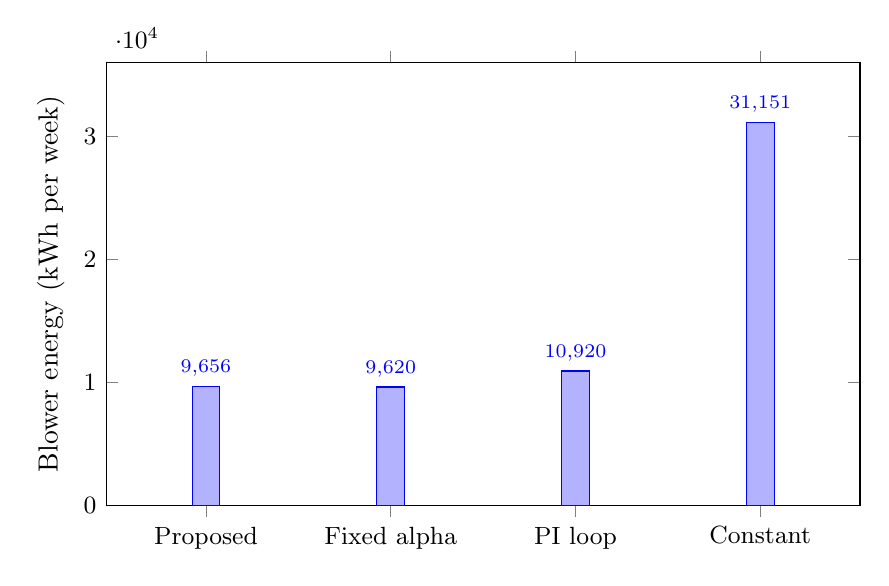
\begin{tikzpicture}
\begin{axis}[
  ybar,
  bar width=10pt,
  width=0.92\textwidth,
  height=7.2cm,
  ylabel={Blower energy (kWh per week)},
  symbolic x coords={Proposed, Fixed alpha, PI loop, Constant},
  xtick=data,
  ymin=0,
  ymax=36000,
  nodes near coords,
  every node near coord/.append style={font=\scriptsize, /pgf/number format/fixed},
  enlarge x limits=0.18,
  tick label style={font=\small}
]
\addplot coordinates {(Proposed,9656) (Fixed alpha,9620) (PI loop,10920) (Constant,31151)};
\end{axis}
\end{tikzpicture}
\caption{Blower electricity over the representative week. The large gap is between constant speed and any loop that moves the fans. The gap between the two predictive laws is not visible at this scale and is discussed with the dissolved-oxygen minima instead.}
\label{fig:energy-bars}
\end{figure}

\subsection{Where the energy is spent}

Table~\ref{tab:regenergy} splits blower energy and mean dissolved oxygen by regime. The proposed loop tracks \eqref{eq:dosp} in every production regime: mean dissolved oxygen is $1.81$, $2.02$, $2.18$, and $2.00\,\mathrm{mg/L}$ against set-points $1.8$, $2.0$, $2.2$, and $2.0$. On the weekend the set-point is $1.3$ but the mean is $4.46\,\mathrm{mg/L}$, because the mixing floor of \SI{900}{\nmcph} delivers more oxygen than the weekend uptake. The floor is doing what it was specified to do. Lowering it to save the weekend kilowatt-hours would put the single online machine on the surge side of \eqref{eq:surge}. The $247\,\mathrm{kWh}$ of the weekend is the price of that constraint, and it is already small next to the fermentation window.

\begin{table}[ht]
\centering
\caption{Blower energy and dissolved oxygen by regime for the proposed loop and the proportional-integral loop.}
\label{tab:regenergy}
\begin{tabular}{@{}lrrrrrr@{}}
\toprule
 & \multicolumn{3}{c}{Proposed} & \multicolumn{3}{c}{Proportional-integral} \\
\cmidrule(lr){2-4} \cmidrule(lr){5-7}
Regime & kWh & mean DO & min DO & kWh & mean DO & min DO \\
\midrule
Base, 96 h & 3469 & 1.81 & 1.72 & 4102 & 2.48 & 1.48 \\
Brewhouse, 30 h & 2438 & 2.02 & 1.39 & 2737 & 2.35 & 2.04 \\
Ferm.\ CIP, 18 h & 2441 & 2.18 & 1.63 & 2460 & 2.21 & 1.87 \\
Pack.\ CIP, 12 h & 1061 & 2.00 & 1.71 & 1318 & 2.61 & 2.33 \\
Weekend, 12 h & 247 & 4.46 & 0.86 & 304 & 5.17 & 2.78 \\
\bottomrule
\end{tabular}
\end{table}

The proportional-integral loop spends $4102-3469=633\,\mathrm{kWh}$ extra on the base regime alone, which is half of its weekly penalty. That is the cost of holding \SI{2.5}{\milli\gram\per\litre} for ninety-six hours when \SI{1.8}{\milli\gram\per\litre} already meets the discharge limit. During fermentation clean-in-place the two loops spend almost the same energy, $2441$ against $2460\,\mathrm{kWh}$, and they hold almost the same mean dissolved oxygen. The detergent window is not where this plant saves energy against a competent fallback. It is where a controller without the right $\alpha$ spends its margin, which is the fixed-$\alpha$ column of Table~\ref{tab:do-cip}.

Mean effluent chemical oxygen demand under the proposed loop is about \SI{56}{\milli\gram\per\litre} in base production, \SI{91}{\milli\gram\per\litre} in the brewhouse peak, \SI{94}{\milli\gram\per\litre} in fermentation clean-in-place, \SI{83}{\milli\gram\per\litre} in packaging clean-in-place, and \SI{39}{\milli\gram\per\litre} on the weekend. The hour-weighted mean is about \SI{67}{\milli\gram\per\litre}. All of these sit under the study limit, with the fermentation window the closest. The limit is not decorative. A longer detergent window, a lower $\alpha$, or a smaller tank would push that \SI{94}{\milli\gram\per\litre} up, and the hinge \eqref{eq:hinge-s} would then start to buy air the energy term does not want. On this week the hinge is inactive. The estimate should say so.

\begin{table}[ht]
\centering
\caption{Fermentation clean-in-place window, where $\alpha$ falls to $0.40$. Minimum dissolved oxygen is the quantity the live transfer estimate is for.}
\label{tab:do-cip}
\begin{tabular}{@{}lrrrr@{}}
\toprule
Loop & kWh in window & Mean DO & Min DO & Mean effluent COD \\
\midrule
Proposed & 2441 & 2.18 & 1.63 & 94 \\
Fixed-$\alpha$ inversion & 2186 & 1.88 & 0.90 & 96 \\
Proportional-integral & 2460 & 2.21 & 1.87 & 93 \\
Constant speed & 3339 & 2.92 & 2.90 & 90 \\
\bottomrule
\end{tabular}
\end{table}

Table~\ref{tab:do-cip} is the case for the second technology. The fixed-$\alpha$ inversion, which is otherwise as economical as the proposed loop, lets dissolved oxygen fall to \SI{0.90}{\milli\gram\per\litre} in the detergent window because it still believes $\alpha=0.55$. The proposed loop, reading $\alpha$ through the $0.30\,\mathrm{h}$ filter, bottoms at \SI{1.63}{\milli\gram\per\litre}. The energy cost of that margin is $2441-2186=255\,\mathrm{kWh}$ inside the window, and across the whole week the two loops differ by only $36\,\mathrm{kWh}$ because the proposed loop saves air in other hours by moving the set-point. A minimum of \SI{0.90}{\milli\gram\per\litre} is above the force-up interlock of \SI{0.4}{\milli\gram\per\litre} and below the operational floor of \SI{1.5}{\milli\gram\per\litre}. It is exactly the region in which nitrification slows, filamentous organisms are selected, and a plant can still post a legal chemical oxygen demand \cite{amand2013review,grady2011,rieger2014abac}. The soft sensor is justified on that floor, not on a kilowatt-hour race against an inversion that was already given a good set-point.

The proportional-integral minimum in the same window is \SI{1.87}{\milli\gram\per\litre}, which also clears the floor. Feedback can find the air if the integrator is allowed to move and the header has capacity. The price is the set-point it was given, paid mostly in the ninety-six quiet hours. The schedule-aware law clears the floor without that set-point. Constant speed clears the floor by a larger margin and pays \SI{3339}{\kilo\watt\hour} in a window where \SI{2441}{\kilo\watt\hour} is enough, and then keeps paying after the window has ended.

One minimum in Table~\ref{tab:regenergy} needs a plain reading. The proposed loop touches \SI{0.86}{\milli\gram\per\litre} on the weekend transition. The weekend mean is \SI{4.46}{\milli\gram\per\litre}, so the touch is a short transient as the load collapses and the bias \eqref{eq:bias} has not yet released the previous airflow command through the blower lag. It is a real defect of the deployed law at regime boundaries that cut the load, not a defect of the sensor. A practical correction, which the estimation did not turn on, is to allow $\sigma$ in \eqref{eq:scale} to fall below one when the previewed load is smaller, clipped for example at $0.7$. The upward clip at $1.35$ was written to avoid over-prediction. The missing downward clip is the weekend transient. It does not create a chemical-oxygen-demand violation on this week. It does cross the weekend floor of \SI{1.0}{\milli\gram\per\litre} briefly. The correction belongs in the next build of the edge image, and it is recorded here so the table is not tidied up after the fact.

\subsection{Exhaust fans and the combined fan account}

Equation~\eqref{eq:exhaust} at the regime speed fractions gives the exhaust-fan power: $6.33\,\mathrm{kW}$ in base production ($0.75^{3}\times 15\,\mathrm{kW}$), $9.21\,\mathrm{kW}$ in the brewhouse peak, $12.86\,\mathrm{kW}$ in both clean-in-place windows, and $2.49\,\mathrm{kW}$ on the weekend. The week is
\begin{equation}
\begin{aligned}
&6.33\times 96
+
9.21\times 30
+
12.86\times 18
+
12.86\times 12
+
2.49\times 12
\\
&\quad
=
608+276+232+154+30
=
1300\,\mathrm{kWh}.
\end{aligned}
\end{equation}
Added to the proposed blower total, the cleaning plant's fans use $9656+1300=10956\,\mathrm{kWh}$ in the week, of which the exhaust share is $12\%$. The exhaust schedule does not depend on which blower loop is selected. Reporting it separately keeps the $11.6\%$ and $69\%$ figures attached to the blowers, which are the machines the two technologies actually move. A combined percentage that mixed a fixed exhaust load into a blower saving would look smaller and would be worse arithmetic.

\subsection{Sensitivity the week already contains}

Three sensitivities are visible without a new plant model.

The mixing floor. Weekend blower energy is $247\,\mathrm{kWh}$ at a mean power of $20.6\,\mathrm{kW}$ even though the uptake would accept less air. Removing the floor would save that energy and would violate \eqref{eq:surge} for a single machine near \SI{2800}{\nmcph} rated flow. The floor stays.

The set-point habit. Moving the proportional-integral set-point from $2.5$ to the schedule \eqref{eq:dosp} would remove most of the $1264\,\mathrm{kWh}$ gap without a soft sensor. That experiment was not the baseline, because the fallback specified in Section~\ref{sec:build} is the habit, not the oracle. It is still the right operational remark: part of technology~1 is the set-point table, and it can be installed even if technology~2 is late.

The $\alpha$ error. Locking $\alpha$ at $0.55$ when the truth is $0.40$ is a relative error of $0.15/0.40=37.5\%$ on the transfer coefficient. The airflow inversion scales as $\alpha^{\,-1/0.82}$, so the missing air fraction before the bias integrator catches up is of order
\begin{equation}
\left(\frac{0.55}{0.40}\right)^{1/0.82}
-
1
=
1.375^{1.220}
-
1
\approx
0.47.
\end{equation}
A forty-seven percent air deficit, held for a fraction of an hour by the blower lag and the bias speed $K_{b}=0.55\,\mathrm{h^{-1}}$, is enough to mark the \SI{0.90}{\milli\gram\per\litre} minimum in Table~\ref{tab:do-cip}. The same arithmetic says what a worse detergent would do. At $\alpha=0.30$ the deficit factor becomes $(0.55/0.30)^{1.220}-1\approx 1.15$, and the header may hit $q_{\max}$ before the set-point is recovered. That case is outside the integrated week. It is the case in which the health bit and the table value in \eqref{eq:alpha-fuse} matter most, because the table for the fermentation recipe is $0.40$, already closer to the truth than the quiet-week $0.55$.

Calendar lead time. The preview of $0.75\,\mathrm{h}$ is several times the blower lag of $0.10\,\mathrm{h}$. Shortening it toward the lag would leave the minimum dissolved oxygen of the proposed loop closer to the fixed-$\alpha$ minimum. Lengthening it beyond the accuracy of the production clock would apply $\sigma>1$ too early and spend air the hinge does not require. The $0.75\,\mathrm{h}$ value is matched to the lags in the model. A site with a slower header should lengthen it, and should do so by measuring the header, not by copying the number.

\subsection{What the estimate does not show}

The integrator does not show a trained network's residual, a drifting diffuser $k_{0}$, a clarifier failure, an anaerobic upset beyond the influent table, a wrong recipe name, or a price that changes inside the week. It does not show three machines of unequal size, where the staging rule \eqref{eq:stage-rule} would be replaced by the integer program. It does not show a permit on suspended solids. It does not show that every brewery will save eleven percent against its existing loop. A plant that already runs ammonia-based aeration control at a low dissolved-oxygen set-point has less left to save against the proportional-integral column and still has the constant-speed column if any tank is in manual \cite{rieger2014abac,amand2012optimal,longo2016}.

Measurement uncertainty on the integrated comparison is the uncertainty of the parameters in \eqref{eq:kla-est} and \eqref{eq:dp-num}, not a Monte Carlo band around a stochastic influent. Those parameters were chosen so the quiet week and the detergent week are both oxygen-feasible. A diffuser whose clean-water $k_{\mathrm{ref}}$ is far below $6.5\,\mathrm{h^{-1}}$ would change the absolute power and could make the fermentation window infeasible at $n=3$. The acceptance test in commissioning is the hand inversion of Section~\ref{sec:saempc} against a measured header, plus one off-gas traverse on a detergent day \cite{asce2007oxygen,leu2009,gillot2005}. If the hand inversion and the meter disagree, the table in this chapter is not a forecast for that header.

Within those limits the estimate supports four sentences. Any of the three modulating loops cuts blower energy by about two thirds relative to constant speed sized for the detergent hour. The schedule-aware set-points cut about twelve percent relative to a competent proportional-integral loop parked at \SI{2.5}{\milli\gram\per\litre}, with no increase in hours above the study chemical-oxygen-demand limit. A predictive inversion without a live $\alpha$ matches that energy and gives up dissolved-oxygen floor during the detergent window, down to \SI{0.90}{\milli\gram\per\litre} against \SI{1.63}{\milli\gram\per\litre}. Exhaust fans add about \SI{1300}{\kilo\watt\hour} in the week under a calendar speed fraction and are not where the saving is. Those four sentences are the quantitative claim of the thesis.

\subsection{Implementation order}

A plant that accepted the specification would not install both technologies on the same day. The order implied by the estimate is the order of the tables. First, move constant-speed tanks onto the Level~1 proportional-integral fallback and confirm the interlocks. That step takes the large share of the energy and does not require an edge computer. Second, install the set-point table \eqref{eq:dosp} and the calendar subscription, still with $\alpha$ from the regime table rather than from the network. Table~\ref{tab:week} says this is where the remaining energy is. Third, train and commission the soft sensor against off-gas on a detergent day, and only then close \eqref{eq:alpha-fuse}. The third step is what protects the dissolved-oxygen floor when the detergent is worse than the table. Building them in the reverse order would put a network in the loop before the plant has a fallback worth falling back to.

The software image of the edge computer should be small enough to review: the inversion, the staging rule, the bias clamp, the health bit, and the log. The full horizon integer program can replace the staging rule when the machines stop being identical, and it should be validated against the rule on the identical-machine case before it is allowed to start a fan the rule would leave off. That validation is a regression test on recorded weeks, not a new theory. The theory this plant needs was already in the aeration-control and predictive-control literature cited in Chapter~\ref{ch:previous}. The part that was not in that literature is the use of the brewery calendar as the disturbance and the use of a transfer residual as the way $\alpha$ enters the fan command. The week integrated here is the estimate of what those two uses are worth when the sensor is good and the calendar is right.

\section{Regime account, boundary dips, and commissioning}
\label{sec:account}

The week totals in Table~\ref{tab:week} are the right summary and a poor diagnosis. A saving that is entirely in one regime is a different design decision from a saving that is spread across the quiet hours. This section writes the four loops regime by regime, using the same integrator, and then states the checks a site would run before the edge computer is allowed to start a fan.

\subsection{All four loops on every regime}

Table~\ref{tab:allreg} extends Table~\ref{tab:regenergy} and Table~\ref{tab:do-cip} to every loop. Energies are blower kilowatt-hours inside the regime. Dissolved oxygen and effluent chemical oxygen demand are time averages inside the regime. The minima are the lowest sample of the $0.02\,\mathrm{h}$ grid, so a one-sample spike is visible and is not averaged away.

\begin{table}[ht]
\centering
\caption{Regime account for all four loops. COD is mean effluent chemical oxygen demand in milligrams per litre. DO is in milligrams per litre.}
\label{tab:allreg}
\scriptsize
\begin{tabular}{@{}llrrrr@{}}
\toprule
Regime & Loop & kWh & mean DO & min DO & mean COD \\
\midrule
Base & Proposed & 3469 & 1.81 & 1.72 & 56 \\
 & Fixed $\alpha$ & 3630 & 2.01 & 1.78 & 56 \\
 & PI & 4102 & 2.48 & 1.48 & 55 \\
 & Constant & 17798 & 5.54 & 2.02 & 52 \\
Brewhouse & Proposed & 2438 & 2.02 & 1.39 & 91 \\
 & Fixed $\alpha$ & 2398 & 1.97 & 1.35 & 91 \\
 & PI & 2737 & 2.35 & 2.04 & 89 \\
 & Constant & 5565 & 3.97 & 3.87 & 84 \\
Ferm.\ CIP & Proposed & 2441 & 2.18 & 1.63 & 94 \\
 & Fixed $\alpha$ & 2186 & 1.88 & 0.90 & 96 \\
 & PI & 2460 & 2.21 & 1.87 & 93 \\
 & Constant & 3339 & 2.92 & 2.90 & 90 \\
Pack.\ CIP & Proposed & 1061 & 2.00 & 1.71 & 83 \\
 & Fixed $\alpha$ & 1113 & 2.11 & 2.00 & 83 \\
 & PI & 1318 & 2.61 & 2.33 & 81 \\
 & Constant & 2222 & 3.78 & 2.99 & 78 \\
Weekend & Proposed & 247 & 4.46 & 0.86 & 39 \\
 & Fixed $\alpha$ & 294 & 4.95 & 2.21 & 39 \\
 & PI & 304 & 5.17 & 2.78 & 38 \\
 & Constant & 2226 & 7.03 & 4.13 & 38 \\
\bottomrule
\end{tabular}
\end{table}

Reading down the energy column, constant speed is the outlier in every regime, including the fermentation window it was sized for. In that window it still uses $3339/2441-1=37\%$ more blower energy than the proposed loop, because a fixed flow sized with a fifteen-percent margin and a slightly different uptake does not land on the inversion the proposed loop recomputes every minute. The quiet base regime is where constant speed is most wrong: $17798$ against $3469\,\mathrm{kWh}$, a factor of about five, for a mean dissolved oxygen of $5.54\,\mathrm{mg/L}$ that the biomass does not use. The weekend is the same pattern on a shorter clock, $2226$ against $247\,\mathrm{kWh}$.

Reading across the minima, two dips belong to the proposed loop and should not be smoothed in a summary. At the entry to the brewhouse peak the proposed minimum is \SI{1.39}{\milli\gram\per\litre}, just under the production floor of \SI{1.5}{\milli\gram\per\litre}. The fixed-$\alpha$ loop dips to \SI{1.35}{\milli\gram\per\litre} at the same boundary. The proportional-integral loop does not, because it is already holding a higher set-point and therefore has air in hand when the load rises. The dip is a preview that is a little late relative to the size of the step from base to brewhouse, not a failure of $\alpha$, which only moves from $0.60$ to $0.52$ at that boundary. Lengthening the lead from $0.75\,\mathrm{h}$ to about $1.5\,\mathrm{h}$ on large upward load steps, while keeping $0.75\,\mathrm{h}$ on detergent steps whose timing is sharper, is the correction consistent with this row. It was not re-integrated. The table is the evidence that the correction is worth doing, and also that the dip does not push mean effluent chemical oxygen demand over the study limit: the brewhouse mean remains \SI{91}{\milli\gram\per\litre}.

The second dip is the weekend entry already noted, \SI{0.86}{\milli\gram\per\litre}, while the weekend mean is \SI{4.46}{\milli\gram\per\litre} because the mixing floor then over-aerates. The fixed-$\alpha$ loop and the proportional-integral loop do not show that particular dip. Their set-points do not fall at the weekend, so they do not have to unload a bias that was supporting a clean-in-place. The proposed loop's lower weekend set-point is still the correct energy decision on the mean. The transient says the unload should be scheduled, by allowing the load scale to drop below one when the previewed mass load falls, rather than discovered by the bias after dissolved oxygen has already risen and then, at the moment of the step, before the blower has slowed. Both dips are properties of the deployed inversion. A horizon formulation of \eqref{eq:p1} that penalizes $\phi_{C}$ inside the horizon would see the weekend unload and the brewhouse rise as future constraints and would move earlier. That is the concrete reason to keep the full economic problem as the specification even though the tables were produced by Algorithm~\ref{alg:deployed}.

The fermentation window remains the row that separates the soft sensor from a good set-point. Mean energies of the proposed loop and the proportional-integral loop are almost equal. Mean chemical oxygen demand values are all legal and within a few milligrams per litre of each other. The minimum dissolved oxygen is not: $1.63$ with the live factor, $0.90$ with $\alpha$ locked at $0.55$, $1.87$ with the high set-point, $2.90$ with constant speed. A report that quoted only kilowatt-hours would rank the fixed-$\alpha$ inversion first in this window, at $2186\,\mathrm{kWh}$, and would be ranking a loop that crossed the operational floor. The separate columns are the reason that ranking is rejected.

\subsection{Mass and energy identities}

The identities below are checks on the tables, not new results. Anyone recomputing the week should recover them before comparing a new controller.

Regime energies of the proposed loop sum as
\begin{equation}
3469+2438+2441+1061+247
=
9656\,\mathrm{kWh},
\end{equation}
which matches Table~\ref{tab:week}. The proportional-integral sum is $4102+2737+2460+1318+304=10921\,\mathrm{kWh}$, against $10920$ in the week table. The one kilowatt-hour is rounding of the regime means. Constant speed sums to $17798+5565+3339+2222+2226=31150\,\mathrm{kWh}$, against $31151$. Specific energy at $9330\,\mathrm{m^{3}}$ is $9656/9330=1.035\,\mathrm{kWh/m^{3}}$ for the proposed blowers. Adding the exhaust account of $1300\,\mathrm{kWh}$ gives $(9656+1300)/9330=1.17\,\mathrm{kWh/m^{3}}$ for every fan on the cleaning plant under the proposed blower law. The proportional-integral plant, with the same exhaust, is $(10920+1300)/9330=1.31\,\mathrm{kWh/m^{3}}$. The constant-speed plant is $(31151+1300)/9330=3.48\,\mathrm{kWh/m^{3}}$. The exhaust addition does not change which loop is cheaper. It stops a later summary from quoting blower-only figures as if the exhaust fans were free.

Effluent chemical oxygen demand under the proposed loop, weighted by hours, is
\begin{equation}
\frac{
56.3\times 96
+
90.9\times 30
+
93.8\times 18
+
83.1\times 12
+
39.3\times 12
}{168}
\approx
67\,\mathrm{mg/L}.
\end{equation}
The influent flow-weighted mean is $3747\,\mathrm{kg}$ over $9330\,\mathrm{m^{3}}$, or \SI{402}{\milli\gram\per\litre}. Removal of total chemical oxygen demand is $1-67/402=0.83$. The inert fraction is $0.08$, so the biodegradable removal is larger than $0.83$ and is not a separate claim. The study limit is \SI{125}{\milli\gram\per\litre}. The margin on the week-average is large. The margin on the fermentation mean, $125-94=31\,\mathrm{mg/L}$, is the one that would disappear first if $\alpha$ were lower or the tank smaller. Design attention belongs on that margin, not on the week-average.

\subsection{Commissioning sequence tied to the tables}

Commissioning follows the implementation order already given, with a measurement at each step so that Table~\ref{tab:allreg} can be rejected or kept.

The first measurement is the header. With one machine online, a technician records airflow, power, and header pressure at three speeds that the drive will actually use, for example speed fractions near $0.55$, $0.75$, and $0.95$. Those three points are compared with Table~\ref{tab:powermap}. A site whose middle point is far from the table replaces $\eta$ and the friction coefficient in \eqref{eq:dp-num} before any controller is judged. Comparing controllers on a wrong power map produces a precise ranking of the wrong plant. The fan test standard is the right experimental frame for this measurement \cite{amca210,dixon2014turbo,iec60034}. The thesis table is only the model those measurements have to beat.

The second measurement is a clean-water or off-gas transfer test at one airflow near \SI{2500}{\nmcph}, which identifies $k_{\mathrm{ref}}$ in \eqref{eq:kla-est} \cite{asce2007oxygen,gillot2005,redmon1983}. If the identified $k_{\mathrm{ref}}$ is not near $6.5\,\mathrm{h^{-1}}$, the inversion \eqref{eq:invert} is wrong by that ratio to the power $1/0.82$, and every airflow command scales. This is a one-day test. It is not optional, because the rest of the estimate is a ratio of controllers that share the same $k_{\mathrm{ref}}$. The ratio can survive a biased $k_{\mathrm{ref}}$. The absolute kilowatt-hours cannot.

The third measurement is a detergent day with the proportional-integral fallback still in charge and the edge computer logging only. The log must show the calendar flag, the dissolved-oxygen minimum, and a portable check of the probe. That day sets the sensor threshold $\epsilon$ and the regime-table value of $\alpha$ for the recipe. If the portable probe and the installed probe disagree by more than a few tenths of a milligram per litre, the bias clamp in \eqref{eq:bias} is reviewed before the edge computer is allowed to write a set-point. The literature on sensor properties is the reason this day exists \cite{rieger2003sensors,olsson2012ica,haimi2013soft}.

The fourth measurement is the first week in which Algorithm~\ref{alg:deployed} writes commands, with Level~1 still able to fall back on a single switch. The week is accepted if three statements hold. Blower energy is below the proportional-integral week on the same production calendar, not below a week of different batches. Hours above the site permit are not higher than the fallback week. The dissolved-oxygen minimum during each detergent recipe stays above the operational floor the site has written down, which in this study is \SI{1.5}{\milli\gram\per\litre}. A site that copies the numbers $11.6\%$ and $69\%$ without those three statements has copied the wrong result. The percentages are the output of one integrator on Table~\ref{tab:regimes}. The three statements are the result that travels.

\subsection{What would falsify the estimate}

The estimate is falsified, for this train, by any of the following observations, and each one points at a specific equation rather than at a vague model error.

If, at the recorded airflows, the power meter disagrees with Table~\ref{tab:powermap} by more than the efficiency uncertainty, then \eqref{eq:polytropic} or \eqref{eq:dp-num} is the wrong header and the kilowatt-hours move. The ranking against constant speed will usually survive, because constant speed is the same wrong map evaluated at one flow. The ranking against the proportional-integral loop is more fragile, because that gap is only twelve percent.

If a detergent day drives $\alpha$ well below the $0.40$ of Table~\ref{tab:regimes} and the third machine at $q_{\max}$ cannot hold the dissolved-oxygen floor, then the plant is oxygen-infeasible and no supervisory law inside this thesis repairs it. The remedy is a diffuser change, a lower load, or a fourth machine \cite{rosso2006alpha,mueller2002aeration,rosso2008state}. Reporting a controller saving on an infeasible plant is not a result.

If the production clock is routinely wrong by more than the preview, the proposed loop collapses toward the fixed-$\alpha$ row of Table~\ref{tab:allreg} whenever the recipe flag is also wrong, and toward a set-point-tracking inversion when only the time is wrong. The dissolved-oxygen minimum in the fermentation window is the first place that collapse would show.

If the clarifier, which this estimate does not model dynamically, loses solids and the permit that actually binds is suspended solids rather than chemical oxygen demand, then the indices in Section~\ref{sec:problem} are the wrong indices \cite{takacs1991,tchobanoglous2014}. The fan law can still be the right fan law. The claim about discharge compliance cannot be carried across that change of permit.

Within the observations the integrator did produce, none of those falsifiers is triggered. Power at the constant-speed flow matches Table~\ref{tab:powermap}. The fermentation window is feasible at a mean near \SI{136}{\kilo\watt}, inside a three-machine header whose constant-speed point is \SI{186}{\kilo\watt}. The calendar in the integrator is the calendar the controller sees. The permit in the integrator is chemical oxygen demand, and the hours above \SI{125}{\milli\gram\per\litre} are zero for every loop. The remaining engineering fact is the one the two technologies were built for. Constant-speed fans sized for the worst hour of a brewery week waste most of their electricity on the other hours. A dissolved-oxygen loop removes most of that waste and leaves a smaller waste that comes from a high, fixed set-point. A schedule-aware inversion removes that smaller waste. A live oxygen-transfer factor does not stack another large energy cut on top of a good set-point. It is what keeps the dissolved-oxygen floor intact when the cleaning chemicals that the brewery must use arrive in the tank the fans are trying to aerate.

\subsection{Open-loop step against the closed-loop week}

Table~\ref{tab:openloop} holds uptake fixed and holds airflow fixed, and it is not a row of Table~\ref{tab:allreg}. The comparison is still the right last check on the estimation, because a reader can otherwise think that a minimum of \SI{0.90}{\milli\gram\per\litre} in the fixed-$\alpha$ loop contradicts an open-loop end point of \SI{0.53}{\milli\gram\per\litre}. It does not. The open-loop step assumes the biomass keeps consuming \SI{30}{\milli\gram\per\litre\per\hour} after dissolved oxygen has collapsed. The week model multiplies the rate by $\mu_{C}=C/(K_{\mathrm{DO}}+C)$. At $C=0.9$ and $K_{\mathrm{DO}}=0.35$ that factor is $0.9/1.25=0.72$, so uptake has already fallen by more than a quarter, the driving force $C^{*}-C$ has widened, and the bias has started to add air. All three effects slow the fall. The open-loop table is the unmitigated error. The week minimum is the error after mitigation by physics the controller does not deserve credit for, plus mitigation by the bias, which it does.

What the controller does deserve credit for is the gap between \SI{0.90}{\milli\gram\per\litre} and \SI{1.63}{\milli\gram\per\litre} in the same window, at nearly the same energy as a predictive law that was handed a sensible set-point and a wrong factor. The proportional-integral minimum of \SI{1.87}{\milli\gram\per\litre} shows that feedback with a high set-point can also clear the floor. It pays for that clearance in the base regime, $4102$ against $3469\,\mathrm{kWh}$. The schedule-aware law clears the floor in the detergent window without paying the quiet-hour price of a permanent \SI{2.5}{\milli\gram\per\litre} set-point. That sentence is the estimate. The open-loop column at \SI{3570}{\nmcph} is why the sentence is about $\alpha$ and not only about set-points. A set-point of \SI{2.0}{\milli\gram\per\litre}, computed with the wrong factor, does not become a tank concentration of \SI{2.0}{\milli\gram\per\litre} until the bias has finished a correction of the size Table~\ref{tab:openloop} measures.

The constant-speed column does not need this distinction. At \SI{6552}{\nmcph} the header is above the corrected detergent airflow of about \SI{5250}{\nmcph} for the whole week, which is why its fermentation minimum is \SI{2.90}{\milli\gram\per\litre} and why its base-regime dissolved oxygen sits near \SI{5.5}{\milli\gram\per\litre}. Safety by excess air is real. It is also the \SI{21495}{\kilo\watt\hour} the modulating loops are measured against. A design review that stops at ``the constant-speed plant met the permit'' has stopped before the only question the fans pose, which is how much air the permit actually required in each hour the calendar had already named.


\nocite{*}
\printbibliography[heading=bibintoc,title={References}]

\end{document}
